\documentclass{article}
\usepackage{url}
\usepackage{fullpage}
\usepackage{hevea}
\usepackage{graphicx}

% Make links between references
\usepackage{hyperref}
\newif\ifpdf
\ifx\pdfoutput\undefined
  \pdffalse
\else
  \pdfoutput=1
  \pdftrue
\fi
\ifpdf
  \hypersetup{colorlinks=true, hyperindex=true, citecolor=red, urlcolor=blue}
\fi

\begin{document}

\title{Biopython Tutorial and Cookbook}
\author{Jeff Chang, Brad Chapman, Iddo Friedberg}
\date{Last Update--11 November 2000}

\maketitle
\tableofcontents

\section{Introduction}

\subsection{What is Biopython?}

\subsection{Obtaining and Installing Biopython}

Biopython's internet home is at, naturally enough,  \ahrefurl{\url{http://www.biopython.org}}. This is the home of all things biopython, so it is the best place to start looking around if you are interested. When you feel ready to dive in and start working with the code, you have two choices:

\begin{enumerate}

\item Release code -- We made available both stable and developer's releases on the download page (\ahrefurl{\url{http://www.biopython.org/Download/}}). The stable releases are likely to be more well tested, while the development releases are closer to what is in CVS, and so will probably have more features.

\item CVS -- The current working copy of the Biopython sources is always available via CVS (Concurrent Versions Systems -- \ahrefurl{\url{http://www.cvshome.org/}}). Concise instructions for accessing this copy are available at \ahrefurl{\url{http://cvs.biopython.org}}.

\end{enumerate}

No matter which way you choose, installing Biopython will require the following easy steps.

\subsubsection{Installation}

Biopython uses Distutils, which is the new standard python installation package. Copies are available at \ahrefurl{\url{http://www.python.org/sigs/distutils-sig/download.html}} and Distutils will also come standard with Python 1.6 and future versions (the version that is shipped with alpha versions of 1.6 should work just fine). Distutils will make installation a snap, as you will see in a second.


Now that we've got what we need let's get into the installation: (Warning: These instructions are strongly biased to UNIX type machines. If you are installing on Windows or Mac or some brand of UNIX for which these instructions are not very helpful, please let us know how we can make them better!)

\begin{enumerate}

\item First you need to unpack the distribution. If you got the CVS version, you are all set to go and can skip on ahead. Otherwise, you'll need to unpack it. On UN*X machines, a tar.gz package is provided, which you can unpack with \verb|tar -xzvpf biopython-X.X.tar.gz|. A zip file is also provided for other platforms. XXX Add stuff about rpms once we get them working.

\item Now that everything is unpacked, move into the \verb| biopython*| directory (this will just be \verb|biopython| for CVS users, and will be \verb|biopython-X.X| for those using a packaged download). 

\item Now you are ready for your one step install -- \verb|python setup.py install|. This performs the default install, and will put Biopython into the \verb|site-packages| directory of your python library tree (on my machine this is \verb|/usr/local/python1.5/site-packages|). You will have to have permissions to write to this directory. 

\begin{enumerate}

\item This install requires that you have the python source available. You can check this by looking for \verb|Python.h| and \verb|config.h| in some place like \verb|/usr/local/include/python1.5|.

\item The distutils setup process allows you to do some customization of your install so you don't have to stick everything in the default location (in case you don't have write permissions there, or just want to test Biopython out). You have quite a few choices, which are covered in detail in the distutils installation manual (http://www.python.org/sigs/distutils-sig/doc/inst/inst.html), specifically in the Alternative installation section.

\end{enumerate}

\item That's it! Biopython is installed. Wasn't that easy? Now let's check and make sure it worked properly.

\end{enumerate}

\subsubsection{Making sure it worked}

First, we'll just do a quick test to make sure python. The most important thing is that python can find the biopython installation. Biopython all installs into a top level \verb|Bio| directory, and you want to make sure this is on your\verb| $PYTHONPATH| on UNIX (hmmm, what do you do on other platforms?). If you used the default install, this shouldn't be a problem, but if not, you'll need to set the \verb|PYTHONPATH| with something like \verb|export PYTHONPATH = $PYTHONPATH':/directory/where/you/put/Biopython'|. Now that we think we are ready, fire up your python interpreter and follow allong with the following quick script:

\begin{verbatim}

[chapmanb@taxus chapmanb]# python
Python 1.6a2 (#1, Jul 31 2000, 09:04:26)  [GCC 2.95.2 19991024 (release/franzo)] on linux2
Copyright 1991-1995 Stichting Mathematisch Centrum, Amsterdam
>>> from Bio.Seq import Seq
>>> new_seq = Seq('GATC') 
>>> new_seq[0:2]
Seq('GA', Alphabet())

\end{verbatim}

If this worked properly, then it looks like Biopython is in a happy place where python can find it, so now you might want to do some more rigorous tests. The \verb|Tests| directory inside the distribution contains a number of tests you can run to make sure all of the different parts of biopython are working. These should all work just by running \verb|python test_WhateverTheTestIs.py|. You can also do a run of all of the tests py typing \verb|python br_regrtest.py| in the Tests directory:

\begin{verbatim}
[chapmanb@taxus Tests]# python br_regrtest.py
test_Enzyme
test_Fasta
test_Fasta2
test_File
....
\end{verbatim}


Well, now you've gotten Biopython installed and running, you are probably ready to get working with it, so continue reading...

\subsection{FAQ}

Hmmmm, don't have a FAQ yet since questions we've seen so far are hopefully covered in the info below. If you have anything that should be in a FAQ, please let us know!

\section{Quick Start -- What can you do with Biopython?}

This section is designed to get you started quickly with Biopython, and to give a general overview of what is available and how to use it. All of the examples in this section assume that you have some general working knowledge of python, and that you have successfully installed biopython on your system. If you think you need to brush up on your python, the main python web site provides quick a bit of free documentation to get started with at \ahrefurl{\url{http://www.python.org/doc/}}. 


Since much biological work on the computer involves connecting with databases on the internet, some of the examples will also require a working internet connection in order to run. 


Now that that is all out of the way, let's get into what we can do with Biopython.

\subsection{General overview of what Biopython provides}

As mentioned in the introduction, Biopython is a set of libraries to provide the ability to deal with ''things'' of interest to biologists working on the computer. In general this means that you will need to have at least some programming experience (in python, of course!) or at least an interest in learning to program. Biopython's job is to make your job easier as a programmer by supplying reusable libraries so that you can focus on answering your specific question of interest, instead of focusing on the internals of parsing a particular file format (of course, if you want to help by writing a parser that doesn't exist and contributing it to Biopython, please go ahead!). So Biopython's job is to make you happy!


One thing to note about Biopython is that it often provides multiple ways of ``doing the same thing.'' To me, this can be frustrating since I  often way to just know the one right way to do something. However, this is also a real benefit because it gives you lots of flexibility and control over the libraries. The tutorial helps to show you the common or easy ways to do things so that you can just make things work. To learn more about the alternative possibilities, look into the Cookbook section (which tells you some cools tricks and tips) and the Advanced section (which provides you with as much detail as you'd ever want to know!). 

\subsection{Working with sequences}

Disputedly (of course!), the central object in bioinformatics is the sequence. Thus, we'll start with the Biopython mechanisms for dealing with sequences. When I think of a sequence the first thing that pops into my mind is a string of letters:\verb| 'AGTACACTGGT'| which seems natural since this is the most common way that sequences are seen in biological file formats.  However, a simple string of letters by itself is also very uninformative -- is it a DNA or  protein sequence (okay, a protein with a lot of Alanines, Glycines, Cysteines and Threonines!), what type of organism did it come from, what is so interesting about it, and so on. The challenge in designing a sequence interface is to pick a representation that is informative enough to take into account the more complex information, yet is as lightweight and easy to work with as just a simple sequence.


The approach taken in the Biopython sequence class is to utilize a class that holds more complex information, yet can be manipulated as if it were a simple string. This is accomplished by utliziing operator overloading to make manipulating a sequence object feel like manipulating a python string. The sequence class, referred to simply as Seq,  is defined in the file \verb|Bio/Seq.py.| Let's look at the Seq class deeper to see what it has to offer.


A biopython Seq object has two important attributes:

\begin{enumerate}

\item \verb|data| -- as the name implies, this is the actual sequence data string of the sequence.

\item \verb|alphabet| -- an object describing what the individual characters making up the string ``mean'' and how they should be interpreted.

\end{enumerate}

Clearly the alphabet object is the important thing that is making the Seq object more than just a string. The currently available alphabets for Biopython are defined in the \verb|Bio/Alphabet| module. We'll use the IUPAC alphabets \ahrefurl ({\url{http://www.chem.qmw.ac.uk/iupac/}}) here to deal with some of our favorite objects: DNA, RNA and Proteins.  


\verb|Bio/Alphabet/IUPAC.py| provides basic definitions for proteins, DNA and RNA, but additionally provides the abilitiy to extend and cutomize the basic definitions. For instance, for proteins, there is a basic IUPACProtein class, but there is an additional ExtendedIUPACProtein class providing for the additional elements ``Asx'' (asparagine or aspartic acid), ``Sec'' (selenocysteine), and ``Glx'' (glutamine or glutamic acid). For DNA you've got choices of IUPACUnambiguousDNA, which provides for just the basic letters, IUPACAmbiguousDNA (which provides for ambiguity letters for every possible situation) and ExtenedIUPACDNA, which allows letters for modified bases. Similarly, RNA can be represented by IUPACAmbigousRNA or IUPACUnambigousRNA.


The advantages of having an alphabet class are two fold. First, this gives an idea of the type of information the \verb|data| object contains. Secondly, this provides a means of contraining the information you have in the data object, as a means of type checking.


Now that we know what we are dealing with, let's look at how to utilize this class to do interesting work.


First, create a Sequence object from a string of information we've got. We'll create an unambiougous DNA object:

\begin{verbatim}
>>> from Bio.Alphabet import IUPAC
>>> my_alpha = IUPAC.unambiguous_dna
>>> from Bio.Seq import Seq
>>> my_seq = Seq('GATCGATGGGCCTATATAGGATCGAAAATCGC', my_alpha)
>>> print my_seq
Seq('GATCGATGGGCCTATATAGGATCGAAAATCGC', IUPACUnambiguousDNA())
\end{verbatim}


Even though this is a sequence object, we can deal with it in some ways as if it were a normal python string. For instance, let's get a slice of the sequence.

\begin{verbatim}
>>> my_seq[4:12]
Seq('GATGGGCC', IUPACUnambiguousDNA())
\end{verbatim}

Two things are interesting to note. First, this follows the normal conventions for python sequences.  So the first element of the sequence is 0 (which is normal for computer science, but not so normal for biology). When you do a slice the first item is included (ie. 4 in this case) and the last is excluded (12 in this case), which is the way things work in python, but of course not necessarily the way everyone in the world would expect. The main goal is to stay consistent with what python does. The second thing to notice is that the slice is performed on the sequence data string, but the new object produced retains the alphabet information from the original Seq object.


You can treat the Seq object like the string in many ways:

\begin{verbatim}
>>> len(my_seq)
32
>>> new_seq = my_seq[0:5]
>>> print new_seq
Seq('GATCG', IUPACUnambiguousDNA())
>>> my_seq + new_seq
Seq('GATCGATGGGCCTATATAGGATCGAAAATCGCGATCG', IUPACUnambiguousDNA())
>>> my_seq[5]
'A'
>>> my_seq == new_seq
0
\end{verbatim}

In all of the operations, the alphabet property is maintained. This is very useful in case you accidentally end up trying to do something weird like add a protein sequence and a DNA sequence:

\begin{verbatim}
>>> protein_seq = Seq('EVRNAK', IUPAC.protein)
>>> dna_seq = Seq('ACGT', IUPAC.unambiguous_dna)
>>> protein_seq + dna_seq
Traceback (most recent call last):
  File "<stdin>", line 1, in ?
  File "/usr/local/lib/python1.6/site-packages/Bio/Seq.py", line 42, in __add__
    raise TypeError, ("incompatable alphabets", str(self.alphabet),
TypeError: ('incompatable alphabets', 'IUPACProtein()', 'IUPACUnambiguousDNA()')
\end{verbatim}


And if you are really just need the string to insert into something, this is very easy to extract:

\begin{verbatim}
>>> my_seq.tostring()
'GATCGATGGGCCTATATAGGATCGAAAATCGC'
\end{verbatim} 

The sequence object is not mutable by default, since in many biological applications you want to ensure you are not changing your data:

\begin{verbatim}
>>> my_seq[5] = 'G'
Traceback (most recent call last):
  File "<stdin>", line 1, in ?
AttributeError: 'Seq' instance has no attribute '__setitem__'
\end{verbatim}

However, you can convert it into a mutable sequence and do pretty much anything you want with it:

\begin{verbatim}
>>> mutable_seq = my_seq.tomutable()
>>> print mutable_seq
MutableSeq('GATCGATGGGCCTATATAGGATCGAAAATCGC', IUPACUnambiguousDNA())
>>> mutable_seq[5] = 'T'
>>> print mutable_seq
MutableSeq('GATCGTTGGGCCTATATAGGATCGAAAATCGC', IUPACUnambiguousDNA())
>>> mutable_seq.remove('T')
>>> print mutable_seq
MutableSeq('GACGTTGGGCCTATATAGGATCGAAAATCGC', IUPACUnambiguousDNA())
>>> mutable_seq.reverse()
>>> print mutable_seq
MutableSeq('CGCTAAAAGCTAGGATATATCCGGGTTGCAG', IUPACUnambiguousDNA())
\end{verbatim}

Now that the nature of the sequence object makes some sense, the next thing to look at is what kind of things we can do with a sequence. The \verb|Bio/Tools| directory contains two useful modules to transcribe and translate a sequence object. These tools work based on the alphabet of the sequence. For instance, let's supposed we want to transcribe our \verb|my_seq| object. Remember that this contains an unambiguous alphabet, so to transcribe we would do the following:

\begin{verbatim}
>>> from Bio.Tools import Transcribe
>>> transcriber = Transcribe.unambiguous_transcriber
>>> my_rna_seq = transcriber.transcribe(my_seq)
>>> print my_rna_seq
Seq('GAUCGAUGGGCCUAUAUAGGAUCGAAAAUCGC', IUPACUnambiguousRNA())
\end{verbatim}

The alphabet of the new RNA Seq object is created for free for you, so again, dealing with a Seq object is no more difficult then dealing with a simple string.


You can also reverse transcribe RNA sequences:

\begin{verbatim}
>>> transcriber.back_transcribe(my_rna_seq)
Seq('GATCGATGGGCCTATATAGGATCGAAAATCGC', IUPACUnambiguousDNA())
\end{verbatim}


To translate our DNA object we have quite a few choices. First, we can use any number of translation tables depending on what we know about our DNA sequence. The translation tables available in biopython were taken from information at \ahrefurl{\url{ftp://ncbi.nlm.nih.gov/entrez/misc/data/gc.prt}}. So, you have tons of choices to pick from. For this, let's just focus on two choices: the Standard translation table, and the Translation table for Vertebrate Mitochondriall DNA. These tables are labelled with id numbers 1 and 2, respectively. Now that we know what tables we are looking to get, we're all set to perform a basic translation. First, we need to get our translators that use these tables. Since we are still dealing with our unambiguous DNA object, we want to fetch translators that take this into account:

\begin{verbatim}
>>> from Bio.Tools import Translate
>>> standard_translator = Translate.unambiguous_dna_by_id[1] 
>>> mito_translator = Translate.unambiguous_dna_by_id[2]
\end{verbatim}

Once we've got the proper translators, it's time to go ahead and translate a sequence:

\begin{verbatim}
>>> my_seq = Seq('GCCATTGTAATGGGCCGCTGAAAGGGTGCCCGA', IUPAC.unambiguous_dna)
>>> standard_translator.translate(my_seq)
Seq('AIVMGR*KGAR', IUPACProtein())
>>> mito_translator.translate(my_seq)
Seq('AIVMGRWKGAR', IUPACProtein())
\end{verbatim}

Notice that the default translation will just go ahead and proceed blindly through a stop codon. If you are aware that you are translating some kind of open reading frame and want to just see everything up until the stop codon, this can be easily done with the \verb|translate_to_stop| function:

\begin{verbatim}
>>> standard_translator.translate_to_stop(my_seq)
Seq('AIVMGR', IUPACProtein())
\end{verbatim}

Similar to the transcriber, it is also possible to reverse translate a protein into a DNA sequence:

\begin{verbatim}
>>> my_protein = Seq('AVMGRWKGGRAAG', IUPAC.protein)
>>> standard_translator.back_translate(my_protein)
Seq('GCTGTTATGGGTCGTTGGAAGGGTGGTCGTGCTGCTGGT', IUPACUnambiguousDNA())
\end{verbatim}

This covers the basic features and uses of the Biopython sequence class. There is a more detailed description of the design ideas behind the sequence class in the Advanced section of this tutorial. This class is still under development and comments on the design and use are, of course, very welcome. Now that you've got some idea of what it is like to interact with the Biopython libraries, it's time to delve into the fun, fun world of dealing with biological file formats!

\subsection{A usage example}
\label{sec:orchids}

Before we jump right into parsers and everything else to do with Biopython, let's set up an example to motivate everything we do and make life more interesting. After all, if there wasn't any biology in this tutorial, why would you want you read it?


Since I love plants, I think we're just going to have to have a plant based example (sorry to all the fans of other organisms out there!).  Having just completed a recent trip to our local greenhouse, we've suddenly developed an incredible obsession with Lady Slipper Orchids (if you wonder why take a look at \ahrefurl{\url{http://www.millicentorchids.com/greenhouse/images/papesq01.jpg}}. If that doesn't convince you, you can look at all of the available photos at  \ahrefurl{\url{http://www.millicentorchids.com/greenhouse/indexphoto.htm}}).  Of course, orchids are not only beautiful to look at, they are also extermely interesting for people studying evolution and systematics. So we're thinking about writing a little proposal to do a molecular study of Lady Slipper evolution and would like to see what kind of research has already been done and how we can add to that.


After a little bit of reading up we discover that the Lady Slipper Orchids are in the Orchidaceae family and the Cypripedioideae sub-family and are made up of 5 genera:  \emph{Cypripedium}, \emph{Paphiopedilum}, \emph{Phragmipedium}, \emph{Selenipedium} and \emph{Mexipedium}. That gives us enough information to get started delving for more information. So, let's look at how biopython tools can help us.

\subsection{Parsing biological file formats}

A large part of much bioinformatics work involves dealing with the many types of file formats designed to hold biological data. These files are loaded with interesting biological data, and a special challenge is parsing these files into a format so that you can manipulate them with some kind of programming language. However the task of parsing these files can be frustrated by the fact that the formats can change quite regularly, and that formats may contain small subleties which can break even the most well designed parsers. 

\subsubsection{General parser design}

The biopython solution to these problem is to develop a structured parser framework that is applicable to all of the parsers. The advantages are two fold. First, this allows code reuse between parsers (see \verb|Bio/ParserSupport.py|). Second, this provides a similar framework for all the parsers so that it is relatively easy to jump into the internals of a parser and figure out problems you might be having. 


All of the parsers have two components:

\begin{enumerate}

\item Scanner - The part of the parser that actually does the work or going through the file and extracting useful information. This useful information is converted into Events.

\item Consumer - The consumer does the job of processing the useful information and spitting it out ina format that the programmer can use. The consumer does this by recieving the events created by the scanner.

\end{enumerate}

So, the parser design is event oriented. The general idea is that a scanner will go through and produce events for every item that might be of interest in a file. For instance, let's say we've got the following FASTA formatted entry (edited to fit the page):


\begin{verbatim}
>gi|6273290|gb|AF191664.1|AF191664 Opuntia clavata rpl16 gene; chloroplast gene for...
TATACATTAAAGGAGGGGGATGCGGATAAATGGAAAGGCGAAAGAAAGAAAAAAATGAA
TCTAAATGATATAGGATTCCACTATGTAAGGTCTTTGAATCATATCATAAAAGACAATGTAAT
AAA...
\end{verbatim}

As a scanner moved through a file containing this entry, it would create the following events:
\\
\\
\begin{tabular}{cc}
Event Name & Entry input \\
\hline
begin\_sequence & (as soon as we notice we've got a new \verb|>|) \\
title & \verb+>gi|6273290|gb|AF191664.1|AF191664 Opuntia clavata...+ \\
sequence & \verb|TATACATTAAAGGAGGGGGATGCGGAT...| \\
sequence & \verb|TCTAAATGATATAGGATTCCACTATGTAA...| \\
sequence & \verb|AAA...| (and so on -- you've got the idea!) \\
end\_sequence & (as soon as we reach a blank line after the sequence data) \\

\end{tabular}
\\
\\
So, events are being produced. Big deal, unless we are able to capture these events and do something interesting with them! This is where the consumer comes in. The consumer needs to do two things:

\begin{enumerate}

\item Register itself with the the scanner to let it know that it wants to recieve those events that are being generated.

\item Do something with the events (and the information associated with them).

\end{enumerate}

An example should make it more clear how this works.

\subsubsection{Writing your own consumer}
\label{sec:writing_consumer}

Now it's time to understand our parser framework, and also start looking at our friends, the lady slipper orchids. To start our search, let's just take a look through the nucleotide databases at NCBI, using an Entrez search (\ahrefurl{\url{lhttp://www.ncbi.nlm.nih.gov:80/entrez/query.fcgi?db=Nucleotide}}) for everything mentioning the text Cypripedioideae (this is the subfamily of lady slipper orchids). This search gives us 94 hits, which we save into a FASTA formatted text file.


Now, let's try and use a parser to summarize the type of information we got. To take a simple example, why don't we go through and grab all of the organism names mentioned, to see how many different species of lady slipper orchids are represented in this data.


To do this kind of useful work, we need to do get our hands dirty and write the solution to all of our problems -- a consumer. This is what our consumer implementation to extract the organisms will look like:

\begin{verbatim}
import string
from Bio.ParserSupport import AbstractConsumer

class SpeciesExtractor(AbstractConsumer):

    def __init__(self):
        self.species_list = []

    def title(self, title_info):
        title_atoms = string.split(title_info)
        new_species = title_atoms[1]

        if new_species not in self.species_list:
            self.species_list.append(new_species)
\end{verbatim}

The first thing we do is import the base class which Consumers should derive from, \verb|AbstractConsumer|. This base class does nice things for us like take care of all the sections we aren't interested in. Then we create our personal consumer class by deriving from this base AbstractConsumer class.


Just like any other python class, we define a \verb|__init__| function that will be called when a new instance of the class is created. In the initialization we set a \verb|species_list| class attribute. This will store the species information as the file is parsed, and will allow us to extract this information later on.


Now we come to the function that is really nifty, the \verb|title| function. This function will be called by the Scanner everytime a 'title' event is generated. So, when the Scanner comes to the first line in our example FASTA file:

\begin{verbatim}
>gi|2765658|emb|Z78533.1|CIZ78533 C.irapeanum 5.8S rRNA gene and ITS1 and ITS2 DNA
\end{verbatim}

It will recognize this as a title, and call the \verb|title| function with the \verb|title_info| argument set as the value of the title.


Now that we've captured the title, we want to extract the information from it we are interested in. Looking at the FASTA title info, we notice that the second item in the info string is the organism name. To get this out we can just use the builtin python function \verb|string.split| to split the string at every space, creating the list \verb|title_atoms|. Since the second element of this list is the species name, we then grab this out of the list. Then we simply check to see if the species is already in our current list of organisms, and if not, we add it.


Okay, well that was easy enough -- so now we need to call the Scanner and actual do this work. To do this, we write a little function:

\begin{verbatim}

from Bio.Fasta import Fasta

def extract_organisms(file, num_records):
    scanner = Fasta._Scanner()
    consumer = SpeciesExtractor()

    file_to_parse = open(file, 'r')

    for fasta_record in range(num_records):
        scanner.feed(file_to_parse, consumer)

    file_to_parse.close()

    return handler.species_list

\end{verbatim}

Let's walk though the function step by step. First, we import the Fasta parser from the Biopython library, then we proceed to define our function. It takes two arguments, the FASTA formatted file to parse, and the number of records in the file. It then creates a Scanner for scanning through FASTA files, and a SpeciesExtractor consumer which will get all of the organisms, as we described above.

We then open our file to parse and get it ready to go. All of the Biopython parsers take file handles as inputs. This means that you can pass them any kind of ``file-like'' object. For instance, the \verb|url| library allows to you work with a document on a remote URL as if it was a local file, so you could use this to pass the parser a document somewhere on the net.


Now that we've got the open file, it's time to parse it. The way the parser works is that you call \verb|feed| for every item in the file you want to parse, passing it the file-like object to parse, and the consumer to call back to. So we loop through all records in the file, and scan them, relying on the consumer to deal with the files as appropriate. Finally, once that is all done, we get the \verb|species_list| attribute of the consumer class, containing all of the information extracted and return that.


Whew, with all of that work out of the way, parsing the file will be really easy:

\begin{verbatim}
all_species = extract_organisms("ls_orchid.fasta", 94)
print "number of species:", len(all_species)
print 'species names:', all_species
\end{verbatim}

Running this all as one big program (the program is available as \verb|fasta_consumer.py| in the \verb|Doc/examples| directory) give us the information we desire:

\begin{verbatim}
[chapmanb@taxus examples]# python fasta_consumer.py
number of species: 92
species names: ['C.irapeanum', 'C.californicum', 'C.fasciculatum', 
'C.margaritaceum', 'C.lichiangense', 'C.yatabeanum', 'C.guttatum',
...
\end{verbatim}

\subsubsection{Making it easier}

The last section explained all of the nitty gritty of writing a specialized consumer. The flexibility of being able to write your own consumer is very nice, however for many applications it can be overkill. For a simple application, the nice Biopython folks have provided some useful classes that act more like full parsers. So, for quick and dirty applications, these are what you want to look at. 


One big problem with the parser we used above was that we were required to know the number of elements in the file. This can be pretty impractical for a lot of applications when you just want to parse through a file and look for something. To help deal with this problem, we can use the \verb|Iterator| interface for FASTA files. This interface allows you to not worry about consumers and scanners and all of that jazz, and just march through a file one record at a time. However, doing this requires that the Iterator return some kind of object that you can manipulate to extract the info you want.


To deal with this problem, a very useful class was written into many of the Biopython parsers -- a \verb|RecordParser|, which parses a file into a python class that represents it. For instance, for FASTA files, the Record class is just an object with \verb|title| and \verb|sequence| attributes. 


Let's make all of this talk more concrete by using the Iterator and Record interefaces to do what we did before -- extract a unique list of all species in our FASTA file. First we need to set up our parser and iterator:

\begin{verbatim}
>>> from Bio.Fasta import Fasta
>>> parser = Fasta.RecordParser()
>>> file = open("ls_orchid.fasta")
>>> iterator = Fasta.Iterator(file, parser)
\end{verbatim}

First we create our parser -- a RecordParser that parses a FASTA entry into the Record class representing it. Then we open the file, and create an iterator, and we are ready to start parsing.


Like most iterator interfaces, we retrieve the objects by calling \verb|next()|. When there are no sequences left to parse, \verb|next()| will return \verb|None|, so we know that it is time to stop. To get our first record:

\begin{verbatim}
>>> cur_record = iterator.next()
\end{verbatim}

Let's take a look at the record object. It has sequence and title attributes that we can easily get at:

\begin{verbatim}
>>> dir(cur_record)
['_colwidth', 'sequence', 'title']
>>> print cur_record.title
gi|2765658|emb|Z78533.1|CIZ78533 C.irapeanum 5.8S rRNA gene and ITS1 and ITS2 DN>>> print cur_record.sequence
CGTAACAAGGTTTCCGTAGGTGAACCTGCGGAAGGATCATTGATGAGACCGTGGAATAAACGATCGAGTGAATCCGGA
...
\end{verbatim}

In my opinion, the coolest thing is how easy it is to get the FASTA record right back:

\begin{verbatim}
>>> print cur_record
>gi|2765658|emb|Z78533.1|CIZ78533 C.irapeanum 5.8S rRNA gene and ITS1 and ITS2 DNA
CGTAACAAGGTTTCCGTAGGTGAACCTGCGGAAGGATCATTGATGAGACCGTGGAATAAA
CGATCGAGTGAATCCGGAGGACCGGTGTACTCAGCTCACCGGGGGCATTGCTCCCGTGGT
GACCCTGATTTGTTGTTGGGCCGCCTCGGGAGCGTCCATGGCGGGTTTGAACCTCTAGCC
CGGCGCAGTTTGGGCGCCAAGCCATATGAAAGCATCACCGGCGAATGGCATTGTCTTCCC
CAAAACCCGGAGCGGCGGCGTGCTGTCGCGTGCCCAATGAATTTTGATGACTCTCGCAAA
CGGGAATCTTGGCTCTTTGCATCGGATGGAAGGACGCAGCGAAATGCGATAAGTGGTGTG
AATTGCAAGATCCCGTGAACCATCGAGTCTTTTGAACGCAAGTTGCGCCCGAGGCCATCA
GGCTAAGGGCACGCCTGCTTGGGCGTCGCGCTTCGTCTCTCTCCTGCCAATGCTTGCCCG
GCATACAGCCAGGCCGGCGTGGTGCGGATGTGAAAGATTGGCCCCTTGTGCCTAGGTGCG
GCGGGTCCAAGAGCTGGTGTTTTGATGGCCCGGAACCCGGCAAGAGGTGGACGGATGCTG
GCAGCAGCTGCCGTGCGAATCCCCCATGTTGTCGTGCTTGTCGGACAGGCAGGAGAACCC
TTCCGAACCCCAATGGAGGGCGGTTGACCGCCATTCGGATGTGACCCCAGGTCAGGCGGG
GGCACCCGCTGAGTTTACGC
\end{verbatim}

We can use all of this to do a rewrite of our \verb|extract_organisms| function:

\begin{verbatim}
def extract_organisms(file_to_parse):

    parser = Fasta.RecordParser()
    file = open(file_to_parse, 'r')
    iterator = Fasta.Iterator(file, parser)

    all_species = []
    cur_record = iterator.next()

    while cur_record:
        # extract the info from the title
        title_atoms = string.split(cur_record.title)
        new_species = title_atoms[1]

        # append the new species to the list if it isn't there
        if new_species not in all_species:
            all_species.append(new_species)

        # advance to the next record
        cur_record = iterator.next()

    return all_species
\end{verbatim}

Running this will give us identical results to what we saw earlier. Whether you choose to use this interface or the previous one depends on your needs and what you feel most comfortable with. Hey, Perl isn't the only place where there's more that one way to do things!

\subsubsection{FASTA files as Dictionaries}

The final thing that we'll do with our ubiquitous orchid fasta file is to show how to index it and access it like a database. This is very useful for large files where you only need to access certain elements of the file, and makes for a nice quick 'n dirty database.


Let's index our record via their GenBank accession number, which seems like a useful way to get track of them. To do this, we first need to write a small function which returns accession numbers from a FASTA record (this is the Record class we discussed earlier):

\begin{verbatim}
import string

def get_accession_num(fasta_record):
    title_atoms = string.split(fasta_record.title)

    # all of the accession number information is stuck in the first element
    # and separated by '|'s
    accession_atoms = string.split(title_atoms[0], '|')
 
    # the accession number is the 4th element
    gb_name = accession_atoms[3]

    # strip the version info before returning
    return gb_name[:-2]
\end{verbatim}

Now we need to create an index from this file, which will show us why writing this function was important. The general format for indexing a file is:

\begin{verbatim}
index_file(file_to_index, index_file_to_create, function_to_get_index_key)
\end{verbatim}

The tricky argument is the \verb|function_to_get_index_key|. Basically, this is a reference to a function that can get called and return an element to use as a key. The idea here is that the \verb|index_file| should be general purpose, and there isn't any good way for the Biopython developers to read your mind and know how you want to index your files. So now the \verb|get_accession_num| function above makes a lot of sense!


Using all of this, we can now create an index file and see how it works. First, let's create the index file:

\begin{verbatim}
>>> from Bio.Fasta import Fasta 
>>> Fasta.index_file("ls_orchid.fasta", "my_orchid_dict.idx", get_accession_num)
\end{verbatim}

This creates an index file \verb|my_orchid_dict.idx| based on the input from \verb|ls_orchid.fasta| and indexed by the values returned by our \verb|get_accession_number| function.


Now that we've got the index, we can create an in-memory dictionary to access the file contents using the index:

\begin{verbatim}
>>> from Bio.Alphabet import IUPAC
>>> dna_parser = Fasta.SequenceParser(IUPAC.ambiguous_dna)
>>> orchid_dict = Fasta.Dictionary("my_orchid_dict.idx", dna_parser)
\end{verbatim} 

The dictionary is created from our \verb|my_orchid_dict.idx| file, and returns Sequence objects. The type of objects returned by the index file are based on the second argument passed. This argument should be a parser that the index file will pass the information through before returning it. If no parser is passed, then the dictionary will just return the raw object (ie. exactly as it appears in the file). 


The parser that we pass here is a \verb|SequenceParser| which converts FASTA files into \verb|SeqRecord| objects. The \verb|SequenceParser| takes an argument of the alphabet we should be using for the sequences. Since the parser can't be smart enough to know exactly what it will be parsing, we need to tell it. If no alphabet is provided, then the parser will default to \verb|Alphabet.generic_alphabet|.


Since this is a dictionary, we can look at all of the keys we have available:

\begin{verbatim}
>>> print orchid_dict.keys()
['Z78475', 'Z78519', 'Z78516', 'Z78517', 'Z78514', 'Z78515', 'Z78512', 
 'Z78513', 'Z78510', 'Z78511', 'Z78457', 'Z78456', 'Z78455', 'Z78454', 
...
\end{verbatim} 

We can access a single sequence object via the keys and manipulate the object as a normal \verb|SeqRecord| object:

\begin{verbatim}
>>> seq_record = orchid_dict['Z78475']
>>> print seq_record
<Bio.SeqRecord.SeqRecord instance at 0x102c1f2c>
>>> print seq_record.description
gi|2765600|emb|Z78475.1|PSZ78475 P.supardii 5.8S rRNA gene and ITS1 and ITS2 DNA
>>> print seq_record.seq
Seq('CGTAACAAGGTTTCCGTAGGTGAACCTGCGGAAGGATCATTGTTGAGATCACATAATAAT ...', IUPACAmbiguousDNA())
\end{verbatim}

That easily, we have created a database of our FASTA file that will spit out sequence objects. 


\subsubsection{I love parsing -- please don't stop talking about it!}

Biopython has a lot of parsers, and each has its own little special niches based on the sequence format it is parsing and all of that. The best place to look for information about specific parsers and how to do cool things with them is in the Cookbook section of the Tutorial. If you don't find the information you are looking for, please consider helping out your poor overworked documentors and submitting a cookbook entry about it! (once you figure out how to do it, that is!)


\subsection{Connecting with biological databases}

One of the very common things that you need to do in bioinformatics is extract information from biological databases. It can be quite tedious to access these databases manually, especially if you have a lot of repetitive work to do. Biopython attempts to save you time and energy by making some on-line databases available from python scripts. Currently, Biopython has code to extract information from the following databases:

\begin{itemize}
  \item ExPASy -- \ahrefurl{\url{http://www.expasy.ch/}} See section~\ref{sec:swiss_prot} in the Cookbook for more information.
  \item Entrez from NCBI -- \ahrefurl{\url{http://www.ncbi.nlm.nih.gov/Entrez/}}
  \item PubMed from NCBI -- \ahrefurl{\url{http://www.ncbi.nlm.nih.gov/PubMed/}}. See section~\ref{sec:pub_med} in the Cookbook for example code detailing how to use this.
  \item SCOP -- \ahrefurl{\url{http://scop.mrc-lmb.cam.ac.uk/scop/}}
\end{itemize}

The code is these modules basically makes it easy to write python code that interact with the CGI scripts on these pages, so that you can get results in an easy to deal with format. In some cases, the results can be tightly integrated with the Biopython parsers to make it even easier to extract information.


Here we'll show a simple example of performing a remote Entrez query. More information on the other services is available in the Cookbook, which begins on page~\pageref{sec:cookbook}.


In section~\ref{sec:writing_consumer} of the parsing examples, we talked about using Entrez to search the NCBI nucleotide databases for info on Cypripedioideae, our friends the lady slipper orchids. Now, we'll look at how to automate that process using a python script. For Entrez searching, this is more useful for displaying results then as a tool for getting sequences. The NCBI web site is mostly set up to allow remote queries so that you could write our own local cgi scripts that return information from NCBI pages. For this reason, the results are returned as HTML and it is pretty tough to get a flat file in a quick manner.


In this example, we'll just show how to connect, get the results, and display them in a web browser. First, we'll start by defining our search and how to display the results:

\begin{verbatim}
search_command = 'Search'
search_database = 'Nucleotide'
return_format = 'FASTA'
search_term = 'Cypripedioideae'

my_browser = 'lynx'
\end{verbatim}

The first four terms define the search we are going to do. To use the Entrez module, you'll need to know a bit about how the remote CGI scripts at NCBI work, and you can find out more about this at \ahrefurl{\url{http://www.ncbi.nlm.nih.gov/entrez/query/static/linking.html}}. The final term just describes the browser to display the results in.


Now that we've got this all set up, we can query Entrez and get a handle with the results. This is done with the following code:

\begin{verbatim}
from Bio.WWW import NCBI

result_handle = NCBI.query(search_command, search_database, term = search_term,
                           doptcmdl = return_format)
\end{verbatim}

The query function does all of the work of preparing the CGI script command line and rounding up the HTML results.


Now that we've got the results, we are ready to save them to a file and display them in our browser, which we can do with code like:

\begin{verbatim}
import os

result_file_name = os.path.join(os.getcwd(), 'results.html')
result_file = open(result_file_name, 'w')
result_file.write(result_handle.read())
result_file.close()

if my_browser == 'lynx':
    os.system('lynx -force_html ' + result_file_name)
elif my_browser == 'netscape':
    os.system('netscape file:' + result_file_name)
\end{verbatim}

Snazzy! We can fetch things and display them automatically -- you could use this to quickly set up searches that you want to repeat on a daily basis and check by hand, or to set up a small CGI script to do queries and locally save the results before displaying them (as a kind of lab notebook of our search results). Hopefully whatever your task, the database connectivity code will make things lots easier for you!

\subsection{Other nifty things}

\subsubsection{Alignments}

Biopython contains some code to deal with doing alignments and dealing with different alignment formats. Right now, you can do the following fun things:

\begin{enumerate}
\item Interact with the clustalw alignment program and parse things in clustalw format. Check section~\ref{sec:align_clustal} of the Cookbook for examples of how to use this.

\item Parse and write out alignments in fasta format. 

\item Translate between the different formats we can deal with. The cookbook also has an example of how to do this in section~\ref{sec:align_translate}
\end{enumerate}

Eventually, it would be nice to be able to deal with all of the various alignment formats and also have code to do pairwise alignments simply from within Biopython. These are definately things that are on my wish list!

\subsection{What to do next}

Now that you've made it this far, you hopefully have a good understanding of the basics of Biopython and are ready to start using it for doing useful work. The best thing to do now is to start snooping around in the source code and looking at the automatically generated documentation. 


Once you get a picture of what you want to do, and what libraries in Biopython will do it, you should take a peak at the Cookbook, which may have example code to do something similar to what you want to do. 


If you know what you want to do, but can't figure out how to do it, please feel free to post questions to the main biopython list (biopython@biopython.org). This will not only help us answer your question, it will also allow us to improve the documentation so it can help the next person do what you want to do.


Enjoy the code!

\section{Cookbook -- Cool things to do with it}
\label{sec:cookbook}

\subsection{BLAST}

Hey, everybody loves BLAST right? I mean, geez, how can get it get any easier to do comparisons between one of your sequences and every other sequence in the known world? Heck, if I was writing the code to do that it would probably take about a day and a half to complete, and the results still wouldn't be as good. But, of course, this section isn't about how cool BLAST is, since we already know that. It is about the problem with BLAST -- it can be really difficult to deal with the volume of data generated by large runs, and to automate BLAST runs in general.


Fortunately, the Biopython folks know this only too well, so they've developed lots of tools for dealing with BLAST and making things much easier. This section details how to use these tools and do useful things with 'em. 

\subsubsection{Running BLAST over the internet}

The first step in automating BLASTing is to make everything accessable from python scripts. So, biopython contains code that allows you to run the WWW version of BLAST (\ahrefurl{\url{http://www.ncbi.nlm.nih.gov/BLAST/}}) directly from your python scripts. This is very nice, especially since BLAST can be a real pain to deal with from scripts, especially with the whole BLAST queue thing and the separate results page.


The code to deal with the WWW version of BLAST is found in the \verb|Bio.Blast.NCBIWWW| module, and the \verb|blast| function. Let's say we want to BLAST info we have in a FASTA formatted file against the database. First, we need to get the info in the FASTA file. The easiest way to do this is to use the Fasta iterator to get a record:

\begin{verbatim}
from Bio.Fasta import Fasta

file_for_blast = open('m_cold.fasta', 'r')
f_iterator = Fasta.Iterator(file_for_blast)

f_record = f_iterator.next()
\end{verbatim}

Now that we've got the fasta record, we are ready to blast it. The code to do the simplest possible BLAST (ie. a simple blastn of the FASTA file against all of the non-redundant databases) is:

\begin{verbatim}
from Bio.Blast import NCBIWWW

b_results = NCBIWWW.blast('blastn', 'nr', f_record)
\end{verbatim}

The \verb|blast| function also take a number of other option arguments which are basically analogous to the different parameters you can set on the basic BLAST page (\ahrefurl{\url{http://www.ncbi.nlm.nih.gov/blast/blast.cgi?Jform=0}}), but for this I'll just talk about the first few arguments, which are the most important (and are also non-optional).


The first argument is the blast program to use for the search. The options and descriptions of the programs are available at \ahrefurl{\url{http://www.ncbi.nlm.nih.gov/BLAST/blast_program.html}}. The second argument specifies the databases to search against. Again, the options for this are available on the NCBI web pages at \ahrefurl{\url{http://www.ncbi.nlm.nih.gov/BLAST/blast_databases.html}}. 


After you have set the search options, you just need to pass in your fasta sequence, which is the third argument, and you are all ready to BLAST. Biopython takes care of worrying about when the results are available, and will pause until it can get the results and return them.


Before parsing the results, it is often useful to save them into a file so that you can use them later without having to go back and re-blast everything. I find this especially useful when debugging my code that extracts info from the BLAST files, but it could also be useful just for making backups of things you've done. If you want to save the results returned, and also parse the results, we need to copy the results before saving them, since using \verb|handle.read()| to write the results to the file will result in not having the info in the handle anymore. I use the \verb|copy| module and code like the following to do this:

\begin{verbatim}
import copy

save_file = open('my_blast.out', 'w')
# copy the handle so we can write it out and still have something for parsing
save_handle = copy.deepcopy(b_results)
save_file.write(save_handle.read())
save_file.close()
\end{verbatim}

After this, the results are in the file \verb|my_blast.out| and the variable \verb|b_results| still contains the results in a ready to parse form.


Well, now that we've got the BLAST results, we are ready to do something with them, so this leads us right into the parsing section.

\subsubsection{Parsing the output from the WWW version of BLAST}

The WWW version of BLAST is of course infamous for continually changing the output in a way that will break parsers that deal with it. Because of this, having a centralized parser in libraries such as Biopython is very important, since then you can have multiple people testing and using it and keeping it up to date. This is so much nicer than trying to keep a tool such as this running yourself.


You can get information to parse with the WWW BLAST parser in one of the two ways. The first is to grab the info using the biopython function for dealing with blast -- doing this is described above. The second way is to manually do the BLAST on the NCBI site, and then save the results. In order to have your output in the right format, you need to save the final BLAST page you get (you know, the one with all of the interesting results!) as HTML (ie. do not save as text!) to a file. The important thing is that you do not have to use biopython scripts to fetch the data in order to be able to parse it.


Doing things either of these two ways, you then need to get a handle to the results. In python, a handle is just a nice general way of describing input to any info source so that the info can be retrieved using \verb|read()| and \verb|readline()| functions. This is the type of input the BLAST parser (and the other biopython parsers take). 


If you followed the code above for interacting with BLAST through a script, then you already have \verb|b_results|, which is great for passing to a parser. If you saved the results in a file, then opening up the file with code like the following will get you what you need:

\begin{verbatim}
b_results = open('my_blast_results', 'r')
\end{verbatim}


Now that we've got a handle, we are ready to parse the output. The code to parse it is really quite small:

\begin{verbatim}
from Bio.Blast import NCBIWWW

b_parser = NCBIWWW.BlastParser()
b_record = b_parser.parse(b_results)
\end{verbatim}

What this accomplishes is parsing the BLAST output into a Blast Record class. The section below on the Record class describes what is contained in this class, but in general, it has got everything you might ever want to extract from the output. Right now we'll just show an example of how to get some info out of the BLAST report, but if you want something in particular that is not described here, look at the info on the record class in detail, and take a gander into the code or automatically generated documentation -- the docstrings have lots of good info about what is stored in each piece of information.


To continue with our example, let's just print out some summary info about all hits in our blast report greater than a particular threshold. The following code does this:

\begin{verbatim}
E_VALUE_THRESH = 0.04

for alignment in b_record.alignments:
    for hsp in alignment.hsps:
        if hsp.expect < E_VALUE_THRESH:
            print '****Alignment****'
            print 'sequence:', alignment.title
            print 'length:', alignment.length
            print 'e value:', hsp.expect
            print hsp.query[0:75] + '...'
            print hsp.match[0:75] + '...'
            print hsp.sbjct[0:75] + '...'
\end{verbatim}

This will print out summary reports like the following:

\begin{verbatim}
****Alignment****
sequence: >gb|AF283004.1|AF283004 Arabidopsis thaliana cold acclimation protein WCOR413-like protein
alpha form mRNA, complete cds
length: 783
e value: 0.034
tacttgttgatattggatcgaacaaactggagaaccaacatgctcacgtcacttttagtcccttacatattcctc...
||||||||| | ||||||||||| || ||||  || || |||||||| |||||| |  | |||||||| ||| ||...
tacttgttggtgttggatcgaaccaattggaagacgaatatgctcacatcacttctcattccttacatcttcttc...
\end{verbatim}

Basically, you can do anything you want to with the info in the BLAST report once you have parsed it. This will, of course, depend on what you want to use it for, but hopefully this helps you get started on doing what you need to do!

\subsubsection{The BLAST record class}

An important consideration for extracting information from a BLAST report is the type of objects that the information is stored in. In Biopython, the parsers return \verb|Record| objects, either \verb|Blast| or \verb|PSIBlast| depending on what you are parsing. These objects are defined in \verb|Bio.Blast.Record| and are quite complete.


Here are my attempts at UML class diagrams for the \verb|Blast| and \verb|PSIBlast| record classes. If you are good at UML and see mistakes/improvements that can be made, please let me know. The Blast class diagram is shown in Figure~\ref{fig:blastrecord}.

\begin{htmlonly}
\label{fig:blastrecord}
\imgsrc[width=650, height=750]{images/BlastRecord.png}
\end{htmlonly}

\begin{latexonly}
\begin{figure}[htbp]
\centering
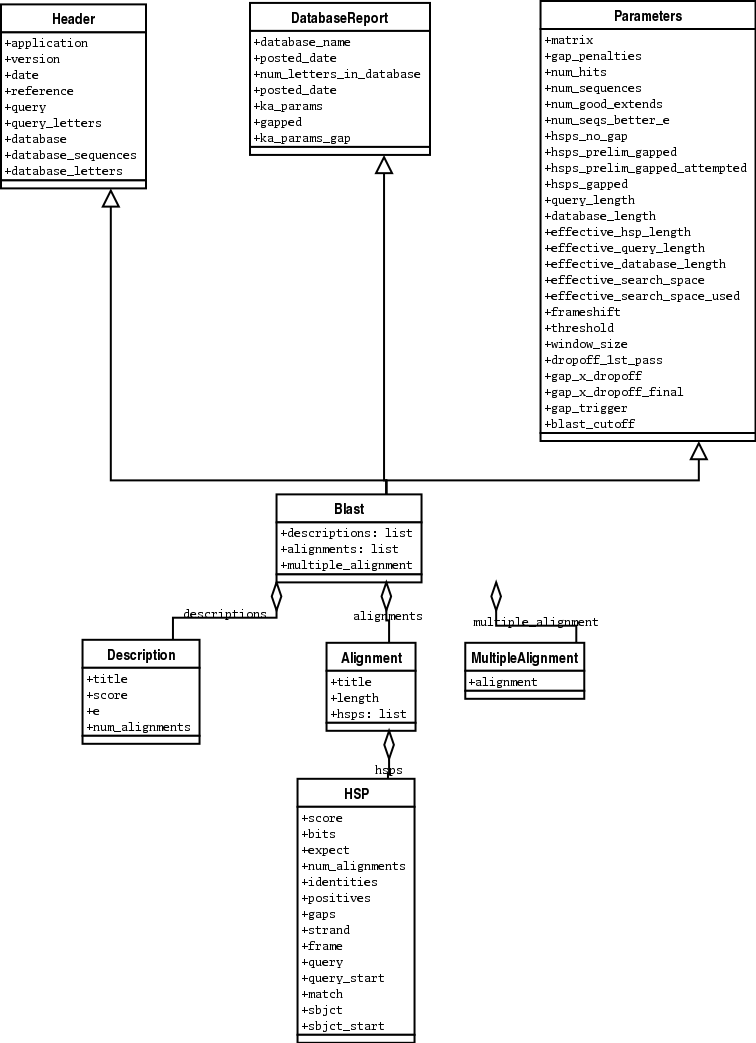
\includegraphics[width=0.8\textwidth]{images/BlastRecord.png}
\caption{Class diagram for the Blast Record class representing all of the info in a BLAST report}
\label{fig:blastrecord}
\end{figure}
\end{latexonly}

The PSIBlast record object is similar, but has support for the rounds that are used in the iteration steps of PSIBlast. The class diagram for PSIBlast is shown in Figure~\ref{fig:psiblastrecord}.

\begin{htmlonly}
\label{fig:psiblastrecord}
\imgsrc[width=650, height=750]{images/PSIBlastRecord.png}
\end{htmlonly}

\begin{latexonly}
\begin{figure}[htbp]
\centering
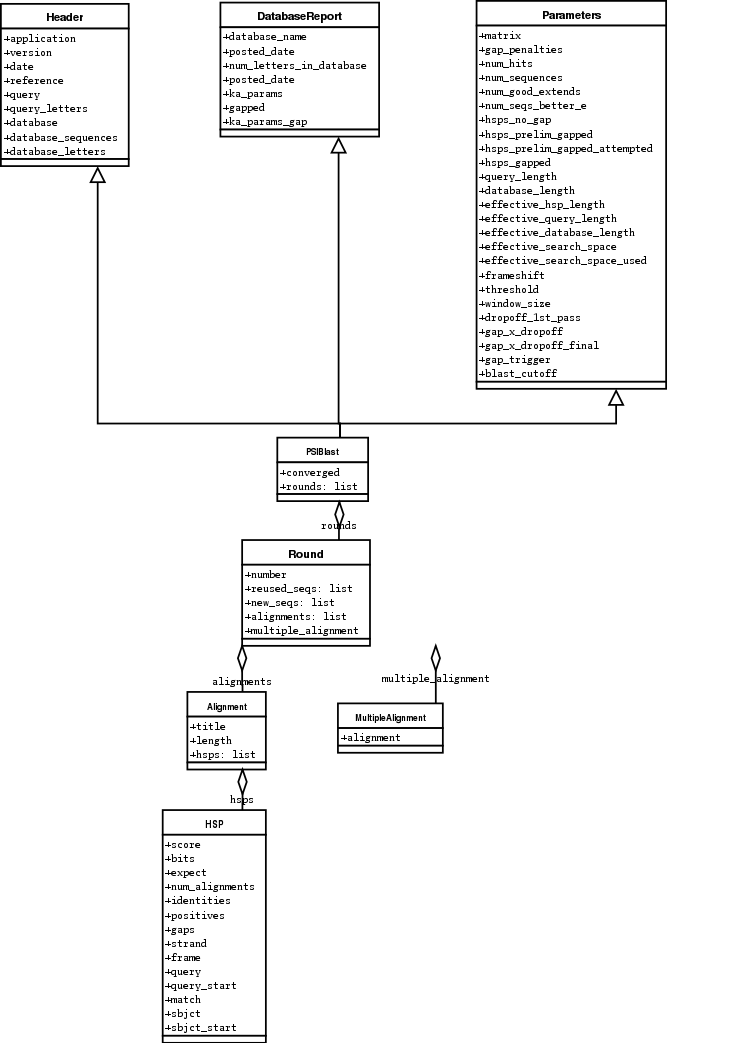
\includegraphics[width=0.8\textwidth]{images/PSIBlastRecord.png}
\caption{Class diagram for the PSIBlast Record class.}
\label{fig:psiblastrecord}
\end{figure}
\end{latexonly}

\subsubsection{Running BLAST locally}

If you want to make your own database to search for sequences against, then local BLAST is definately the way you want to go. As with online BLAST, biopython provides lots of nice code to make you able to call local BLAST executables from your scripts, and have full access to the many command line options that these executables provide. You can obtain local BLAST precompiled for a number of platforms at \ahrefurl{\url{ftp://ncbi.nlm.nih.gov/blast/executables/}}, or can compile it yourself in the NCBI toolbox (\ahrefurl{\url{ftp://ncbi.nlm.nih.gov/toolbox/}}).


The code for dealing with local BLAST is found in \verb|Bio.Blast.NCBIStandalone|, specifically in the functions \verb|blastall| and \verb|blastpgp|, which correspond with the BLAST executables that their names imply.


Let's use these functions to run a \verb|blastall| against a local database and return the results. First, we want to set up the paths to everything that we'll need to do the blast. What we need to know is the path to the database (which should have been prepared using \verb|formatdb|) to search against, the path to the file we want to search, and the path to the \verb|blastall| executable.

\begin{verbatim}
import os

my_blast_db = os.path.join(os.getcwd(), 'at-est', 'a_cds-10-7.fasta')
my_blast_file = os.path.join(os.getcwd(), 'at-est', 'test_blast',
                             'sorghum_est-test.fasta')
my_blast_exe = os.path.join(os.getcwd(), 'blast', 'blastall')
\end{verbatim}

Now that we've got that all set, we are ready to run the blast and collect the results. We can do this with two lines:

\begin{verbatim}
from Bio.Blast import NCBIStandalone

blast_out, error_info = NCBIStandalone.blastall(my_blast_exe, 'blastn',
                                                my_blast_db, my_blast_file)
\end{verbatim}

Note that the biopython interfaces to local blast programs returns two values. The first is a handle to the blast output, which is ready to either be saved or passed to a parser. The second is the possible error output generated by the blast command.


The error info can be hard to deal with, because if you try to do a \verb|error_info.read()| and there was no error info returned, then the \verb|read()| call will block and not return, locking your script. In my opinion, the best way to deal with the error is only to print it out if you are not getting \verb|blast_out| results to be parsed, but otherwise to leave it alone.


If you are interested in saving your results to a file before parsing them, see the section on WWW blast above for some info on how to use the \verb|copy| module to do this.


Well, now that you've got output, we should start parsing them, so read on to learn about parsing local BLAST output.

\subsubsection{Parsing BLAST output from local BLAST}

Since the output generated by local BLAST is different than that generated by the web-based BLAST, we use the parsers located in \verb|Bio.Blast.NCBIStandalone| to parse and deal with the results.


As with WWW blast (see the info on this above) we need to have a handle object that we can pass to the parser. The handle must implement the \verb|readline()| method and do this properly. The common ways to get such a handle are to either use the provided \verb|blastall| or \verb|blastpgp| functions to run the local blast, or to run a local blast via the commandline, and then do something like the following:

\begin{verbatim}
blast_out = open('my_file_of_blast_output', 'r')
\end{verbatim}

So, as with WWW blast, there is no need to use the biopython convenience functions if you don't want to.


Well, now that we've got a handle (which we'll call \verb|blast_out|), we are ready to parse it. This can be done with the following code:

\begin{verbatim}
from Bio.Blast import NCBIStandalone

b_parser = NCBIStandalone.BlastParser()
b_record = b_parser.parse(blast_out)
\end{verbatim} 

This will parse the BLAST report into a Blast Record class (either a Blast or a PSIBlast record, depending on what you are parsing) so that you can extract the information from it. In our case, let's just use print out a quick summary of all of the alignments greater than some threshold value.

\begin{verbatim}
E_VALUE_THRESH = 0.04
for alignment in b_record.alignments:
    for hsp in alignment.hsps:
        if hsp.expect < E_VALUE_THRESH:
            print '****Alignment****'
            print 'sequence:', alignment.title
            print 'length:', alignment.length
            print 'e value:', hsp.expect
            print hsp.query[0:75] + '...'
            print hsp.match[0:75] + '...'
            print hsp.sbjct[0:75] + '...'
\end{verbatim}

If you also read the section on parsing BLAST from the WWW version, you'll notice that the above code is identical to what is found in that section. Once you parse something into a record class you can deal with it independent of the format of the original BLAST info you were parsing. Pretty snazzy!


Sure, parsing one record is great, but I've got a BLAST file with tons of records -- how can I parse them all? Well, fear not, the answer lies in the very next section.

\subsubsection{Parsing a file full of BLAST runs}

Of course, local blast is cool because you can run a whole bunch of sequences against a database and get back a nice report on all of it. So, biopython definately has facilities to make it easy to parse humungous files without memory problems. 


We can do this using the blast iterator. To set up an iterator, we first set up a parser, to parse our blast reports in Blast Record objects:

\begin{verbatim}
from Bio.Blast import NCBIStandalone

b_parser = NCBIStandalone.BlastParser()
\end{verbatim}

Then we will assume we have a handle to a bunch of blast records, which we'll call \verb|blast_out|. Getting a handle is described in full detail above in the blast parsing sections. 


Now that we've got a parser and a handle, we are ready to set up the iterator with the following command:

\begin{verbatim}
b_iterator = NCBIStandalone.Iterator(blast_out, b_parser)
\end{verbatim}

The second option, the parser, is optional. If we don't supply a parser, then the iterator will just return the raw BLAST reports one at a time.


Now that we've got an iterator, we start retrieving blast records (generated by our parser) using \verb|next()|:

\begin{verbatim}
b_record = b_iterator.next()
\end{verbatim}

Each call to next will return a new record that we can deal with. Now we can iterate through this records and generate our old favorite, a nice little blast report:

\begin{verbatim}
while b_record:
    E_VALUE_THRESH = 0.04
    for alignment in b_record.alignments:
        for hsp in alignment.hsps:
            if hsp.expect < E_VALUE_THRESH:
                print '****Alignment****'
                print 'sequence:', alignment.title
                print 'length:', alignment.length
                print 'e value:', hsp.expect

                if len(hsp.query) > 75:
                    dots = '...'
                else:
                    dots = ''
                
                print hsp.query[0:75] + dots
                print hsp.match[0:75] + dots
                print hsp.sbjct[0:75] + dots

    b_record = b_iterator.next()
\end{verbatim}

Notice that \verb|b_iterator.next()| will return \verb|None| when it runs out of records to parse, so it is easy to iterate through the entire file with a while loop that checks for the existance of a record.


The iterator allows you to deal with huge blast records without any memory problems, since things are read in one at a time. I have parsed tremendously huge files without any problems using this.

\subsubsection{Finding a bad record somewhere in a huge file}

One really ugly problem that happens to me is that I'll be parsing a huge blast file for a while, and the parser will bomb out with a SyntaxError. This is a serious problem, since you can't tell if the SyntaxError is due to a parser problem, or a problem with the BLAST. To make it even worse, you have no idea where the parse failed, so you can't just ignore the error, since this could be ignoring an important data point.


We used to have to make a little script to get around this problem, but the \verb|Bio.Blast| module now includes a \verb|BlastErrorParser| which really helps make this easier. The \verb|BlastErrorParser| works very similar to the regular \verb|BlastParser|, but it adds an extra layer of work by catching SyntaxErrors that are generated by the parser, and attempting to diagnose the errors.


Let's take a look at using this parser -- first we define the file we are going to parse and the file to write the problem reports to:

\begin{verbatim}
import os
 
b_file = os.path.join(os.getcwd(), 'blast_out', 'big_blast.out')
error_file = os.path.join(os.getcwd(), 'blast_out', 'big_blast.problems')
\end{verbatim}

Now we want to get a \verb|BlastErrorParser|:

\begin{verbatim}
from Bio.Blast import NCBIStandalone

error_handle = open(error_file, 'w')

b_error_parser = NCBIStandalone.BlastErrorParser(error_handle)
\end{verbatim}

Notice that the parser take an optional argument of a handle. If a handle is passed, then the parser will write any blast records which generate a SyntaxError to this handle. Otherwise, these records will not be recorded.


Now we can use the \verb|BlastErrorParser| just like a regular blast parser. Specifically, we might want to make an iterator that goes through our blast records one at a time and parses them with the error parser:

\begin{verbatim}
blast_out = open(b_file)
iterator = NCBIStandalone.Iterator(blast_out, b_error_parser)
\end{verbatim}

Just like before, we can read these records one a time with, but now we can catch and deal with errors that are due to problems with Blast (and not with the parser itself):

\begin{verbatim}
try:
    next_record = iterator.next()
except NCBIStandalone.LowQualityBlastError, info:
    print "LowQualityBlastError detected in id %s" % info[1]
\end{verbatim}

Right now the \verb|BlastErrorParser| can generate the following errors:

\begin{itemize}
  \item \verb|SyntaxError| -- This is the same error generated by the regular BlastParser, and is due to the parser not being able to parse a specific file. This is normally either due to a bug in the parser, or some kind of descrepency between the version of BLAST you are using and the versions the parser is able to handle.

  \item \verb|LowQualityBlastError| -- When BLASTing a sequence that is of really bad quality (for example, a short sequence that is basically a stretch of one nucleotide), it seems that Blast ends up masking out the entire sequence and ending up with nothing to parse. In this case it will produce a truncated report that causes the parser to generate a SyntaxError. \verb|LowQualityBlastError| is reported in these cases. This error returns an info item with the following information:
  \begin{itemize}
    \item \verb|item[0]| -- The error message
    \item \verb|item[1]| -- The id of the input record that caused the error. This is really useful if you want to record all of the records that are causing problems.
  \end{itemize}
\end{itemize}

As mentioned, with each error generated, the BlastErrorParser will write the offending record to the specified \verb|error_handle|. You can then go ahead and look and these and deal with them as you see fit. Either you will be able to debug the parser with a single blast report, or will find out problems in your blast runs. Either way, it will definately be a useful experience!


Hopefully the \verb|BlastErrorParser| will make it much easier to debug and deal with large Blast files.

\subsubsection{Dealing with PSIBlast}

We should write some stuff to make it easier to deal directly with PSIBlast from scripts (ie. output the align file in the proper format from an alignment). I need to look at PSIBlast more and come up with some good ways of going this...

\subsection{SWISS-PROT}
\label{sec:swiss_prot}

\subsubsection{Retrieving a SWISS-PROT record}

SwissProt (\ahrefurl{\url{http://www.expasy.ch/sprot/sprot-top.html}}) is a handcurated database of protein sequences. Let's look at how we connect with it from a script and parse SwissProt formatted results. 


First, we need to retrieve some results to parse. Let's say we are looking at chalcone synthases for Orchids (see section~\ref{sec:orchids} for some justification for looking for interesting things about orchids). Chalcone synthase is involved in flavanoid biosynthesis in plants, and flavanoids make lots of cool things like pigment colors and UV protectants. 


If you do a search on SwissProt, you can find three orchid proteins for Chalcone Synthase, id numbers O23729, O23730, O23731. Now, let's write a script which grabs these, and parses out some interesting information.


First, we grab the records, using the \verb|get_sprot_raw()| function of \verb|Bio.WWW.Expasy|. This function is very nice since you can feed it an id and get back a raw text record (no html to mess with!). As we get the three records we are interested in, we'll just put them together into one big string, which we'll then use for parsing. The following code accomplishes what I just wrote:

\begin{verbatim}
from Bio.WWW import ExPASy

ids = ['O23729', 'O23730', 'O23731']

all_results = ''
for id in ids:
    results = ExPASy.get_sprot_raw(id)
    all_results = all_results + results.read()
\end{verbatim}

Now that we've got the results, we are ready to parse them into interesting information. As with most parsers, we set up an iterator and parser. The parser we use here parses the SwissProt files into a Record object where the interesting features are attributes:

\begin{verbatim}
from Bio.SwissProt import SProt
from Bio import File

s_parser = SProt.RecordParser()
s_iterator = SProt.Iterator(File.StringHandle(all_results), s_parser)
\end{verbatim}

Note that we convert \verb|all_results|, which is a string, into a handle before passing it. The iterator requires a handle to be passed so that it can read in everything one line at a time. The \verb|Bio.File| module has a nice StringHandle, which conveniently will convert a string into a handle. Very nice! Now we are ready to start extracting information.


To get out the information, we'll go through everything record by record using the iterator. For each record, we'll just print out some summary information:

\begin{verbatim}
cur_record = s_iterator.next()

while cur_record:
    print "description:", cur_record.description
    for ref in cur_record.references:
        print "authors:", ref.authors
        print "title:", ref.title

    print "classification:", cur_record.organism_classification
    print

    cur_record = s_iterator.next()
\end{verbatim}

This prints out a summary like the following:

\begin{verbatim}
description: CHALCONE SYNTHASE 8 (EC 2.3.1.74) (NARINGENIN-CHALCONE SYNTHASE 8)
authors: Liew C.F., Lim S.H., Loh C.S., Goh C.J.;
title: "Molecular cloning and sequence analysis of chalcone synthase cDNAs of
Bromheadia finlaysoniana.";
classification: ['Eukaryota', 'Viridiplantae', 'Embryophyta', 'Tracheophyta', 
'Spermatophyta', 'Magnoliophyta', 'Liliopsida', 'Asparagales', 'Orchidaceae', 
'Bromheadia']
\end{verbatim}

It is equally easy to extract any kind of information you'd like from SwissProt records.

\subsection{PubMed}
\label{sec:pub_med}

\subsubsection{Sending a query to PubMed}

If you are in the Medical field or interested in human issues (and many times even if you are not!), PubMed (\ahrefurl{\url{http://www.ncbi.nlm.nih.gov/PubMed/}}) is an excellent source of all kinds of goodies. So like other things, we'd like to be able to grab information from it and use it in python scripts.


Querying PubMed using Biopython is extremely painless. To get all of the article ids for articles having to do with orchids, we only need the following three lines of code:

\begin{verbatim}
from Bio.Medline import PubMed

search_term = 'orchid'
orchid_ids = PubMed.search_for(search_term)
\end{verbatim}

This returns a python list containing all of the orchid ids

\begin{verbatim}
['11070358', '11064040', '11028023', '10947239', '10938351', '10936520', 
'10905611', '10899814', '10856762', '10854740', '10758893', '10716342', 
...
\end{verbatim}

With this list of ids we are ready to start retrieving the records, so follow on ahead to the next section.

\subsubsection{Retrieving a PubMed record}

The previous section described how to get a bunch of article ids. Now that we've got them, we obviously want to get the corresponding Medline records and extract the information from them. 


The interface for retrieving records from PubMed should be very intuitive to python programmers -- it models a python dictionary. To set up this interface, we need to set up a parser that will parse the results that we retrieve. The following lines of code get everything set up:

\begin{verbatim}
from Bio.Medline import PubMed
from Bio.Medline import Medline

rec_parser = Medline.RecordParser()
medline_dict = PubMed.Dictionary(parser = rec_parser)
\end{verbatim}

What we've done is create a dictionary like object \verb|medline_dict|. To get an article we access it like \verb|medline_dict[id_to_get]|. What this does is connect with PubMed, get the article you ask for, parse it into a record object, and return it. Very cool! 


Now let's look at how to use this nice dictionary to print out some information about some ids. We just need to loop through our ids (\verb|orchid_ids| from the previous section) and print out the information we are interested in:

\begin{verbatim}
for id in orchid_ids[0:5]:
    cur_record = medline_dict[id]
    print 'title:', string.rstrip(cur_record.title)
    print 'authors:', cur_record.authors
    print 'source:', string.strip(cur_record.source)
    print
\end{verbatim}

The output for this looks like:

\begin{verbatim}
title: Sex pheromone mimicry in the early spider orchid (ophrys sphegodes):
patterns of hydrocarbons as the key mechanism for pollination by sexual
deception [In Process Citation]
authors: ['Schiestl FP', 'Ayasse M', 'Paulus HF', 'Lofstedt C', 'Hansson BS', 
'Ibarra F', 'Francke W']
source: J Comp Physiol [A] 2000 Jun;186(6):567-74
\end{verbatim}

Especially interesting to note is the list of authors, which is returned as a standard python list. This makes it easy to manipulate and search using standard python tools. For instance, we could loop through a whole bunch of entries searching for a particular author with code like the following:

\begin{verbatim}
search_author = 'Waits T'

for id in our_id_list:
    cur_record = medline_dict[id]
    
    if search_author in cur_record.authors:
        print "Author %s found: %s" % (search_author,
                                       string.strip(cur_record.source))
\end{verbatim} 

The PubMed and Medline interfaces are very mature and nice to work with -- hopefully this section gave you an idea of the power of the interfaces and how they can be used.

\subsection{Dealing with alignments}

It is often very useful to be able to align particular sequences. I do this quite often to get a quick and dirty idea of relationships between sequences. Consequently, it is very nice to be able to quickly write up a python script that does an alignment and gives you back objects that are easy to work with. The alignment related code in Biopython is meant to allow python-level access to alignment programs so that you can run alignments quickly from within scripts.

\subsubsection{Clustalw}
\label{sec:align_clustal}

Clustalx (\ahrefurl{\url{http://www-igbmc.u-strasbg.fr/BioInfo/ClustalX/Top.html}}) is a very nice program for doing multiple alignments. Biopython offers access to alignments in clustal format (these normally have a \verb|*.aln| extension) that are produced by Clustalx. It also offers access to clustalw, which the is command line version of clustalx.


The first step in interacting with clustalw is to set up a command line you want to pass to the program. Clustalw has a ton of command line options, and if you set a lot of parameters, you can end up typing in a huge ol' command line quite a bit. This command line class models the command line by making all of the options be attributes of the class that can be set. A few convenience functions also exist to set certain parameters, so that some error checking on the parameters can be done.


To create a command line object to do a clustalw multiple alignment we do the following:

\begin{verbatim}
import os
from Align.Clustalw import MultipleAlignCL

cline = MultipleAlignCL(os.path.join(os.curdir, 'opuntia.fasta'))
cline.set_output('test.aln')
\end{verbatim}

First we import the \verb|MultipleAlignCL| object, which models running a multiple alignment from clustalw. We then initialize the command line, with a single argument of the fasta file that we are going to be using for the alignment. The initialization function also takes an optional second argument which specifies the location of the \verb|clustalw| executable. By default, the commandline will just be invoked with 'clustalw,' assuming that you've got it somewhere on your \verb|PATH|.


The second argument sets the output to go to the file \verb|test.aln|. The \verb|MultipleAlignCL| object also has numerous other parameters to specify things like output format, gap costs, etc. 


We can look at the command line we have generated by invoking the \verb|__str__| member attribute of the \verb|MultipleAlignCL| class. This is done by calling \verb|str(cline)| or simple by printing out the command line with \verb|print cline|. In this case, doing this would give the following output:

\begin{verbatim}
clustalw ./opuntia.fasta -OUTFILE=test.aln
\end{verbatim}

Now that we've set up a simple command line, we now want to run the commandline and collect the results so we can deal with them. This can be done using the \verb|do_alignment| function of \verb|Clustalw| as follows:

\begin{verbatim}
from Bio.Clustalw import Clustalw

alignment = Clustalw.do_alignment(cline)
\end{verbatim}

What happens when you run this if that Biopython executes your command line and runs clustalw with the given parameters. It then grabs the output, and if it is in a format that Biopython can parse (currently only clustal format), then it will parse the results and return them as an alignment object of the appropriate type. So in this case since we are getting results in the default clustal format, the returned \verb|alignment| object will be a \verb|ClustalAlignment| type.


Once we've got this alignment, we can do some interesting things with it such as get \verb|seq_record| objects for all of the sequences involved in the alignment:

\begin{verbatim}
all_records = alignment.get_all_seqs()

print 'description:', all_records[0].description
print 'sequence:', all_records[0].seq
\end{verbatim}

This prints out the description and sequence object for the first sequence in the alignment:

\begin{verbatim}
description: gi|6273285|gb|AF191659.1|AF191
sequence: Seq('TATACATTAAAGAAGGGGGATGCGGATAAATGGAAAGGCGAAAGAAAGAAAAAAATGAAT 
...', IUPACAmbiguousDNA())
\end{verbatim}

You can also calculate the maximum length of the alignment with:

\begin{verbatim}
length = alignment.get_alignment_length()
\end{verbatim}

Finally, to write out the alignment object in the original format, we just need to access the \verb|__str__| function. So doing a \verb|print alignment| gives:

\begin{verbatim}
CLUSTAL X (1.81) multiple sequence alignment


gi|6273285|gb|AF191659.1|AF191      TATACATTAAAGAAGGGGGATGCGGATAAATGGAAAGGCGAAAGAAAGAA
gi|6273284|gb|AF191658.1|AF191      TATACATTAAAGAAGGGGGATGCGGATAAATGGAAAGGCGAAAGAAAGAA
...
\end{verbatim}

This makes it easy to write your alignment back into a file with all of the original info intact.


If you want to do more interesting things with an alignment, the best thing to do is to pass the alignment to an alignment information generating object, such as the SummaryInfo object, described in section~\ref{sec:summary_info}.

\subsubsection{Calculating summary information}
\label{sec:summary_info}

Once you have an alignment, you are very likely going to want to find out information about it. Instead of trying to have all of the functions that can generate information about an alignment in the alignment object itself, we've tried to separate out the functionality into separate classes, which act on the alignment. 


Getting ready to calculate summary information about an object is quick to do. Let's say we've got an alignment object called \verb|alignment|. All we need to do to get an object that will calculate summary information is:

\begin{verbatim}
from Bio.Align import AlignInfo
summary_align = AlignInfo.SummaryInfo(alignment)
\end{verbatim}

The \verb|summary_align| object is very useful, and will do the following neat things for you:

\begin{enumerate}
  \item Calculate a quick consensus sequence -- see section~\ref{sec:consensus}
  \item Get a position specific score matrix for the alignment -- see section~\ref{sec:pssm}
  \item Calculate the information content for the alignment -- see section~\ref{sec:getting_info_content}
  \item Generate information on substitutions in the alignment -- section~\ref{sec:sub_matrix} details using this to generate a substitution matrix.
\end{enumerate}

\subsubsection{Calculating a quick consensus sequence}
\label{sec:consensus}

The \verb|SummaryInfo| object, described in section~\ref{sec:summary_info}, provides functionality to calculate a quick consensus of an alignment. Assuming we've got a \verb|SummaryInfo| object called \verb|summary_align| we can calculate a consensus by doing:

\begin{verbatim}
consensus = summary_align.dumb_consensus()
\end{verbatim}

As the name suggests, this is a really simple consensus calculator, and will just add up all of the residues at each point in the consensus, and if the most common value is higher than some threshold value (the default is .3) will add the common residue to the consensus. If it doesn't reach the threshold, it adds an ambiguity character to the consensus. The returned consensus object is Seq object whose alphabet is inferred from the alphabets of the sequences making up the consensus. So doing a \verb|print consensus| would give:

\begin{verbatim}
consensus Seq('TATACATNAAAGNAGGGGGATGCGGATAAATGGAAAGGCGAAAGAAAGAAAAAAATGAAT 
...', IUPACAmbiguousDNA())
\end{verbatim} 

You can adjust how \verb|dumb_consensus| works by passing optional parameters:

\begin{description}
\item[the threshold] This is the threshold specifying how common a particular residue has to be at a position before it is added. The default is .7.

\item[the ambiguous character] This is the ambiguity character to use. The default is 'N'.

\item[the consensus alphabet] This is the alphabet to use for the consensus sequence. If an alphabet is not specified than we will try to guess the alphabet based on the alphabets of the sequences in the alignment.
\end{description}

\subsubsection{Position Specific Score Matrices}
\label{sec:pssm}

Position specific score matrices (PSSMs) summarize the alignment information in a different way than a consensus, and may be useful for different tasks. Basically, a PSSM is a count matrix. For each column in the alignment, the number of each alphabet letters is counted and totaled. The totals are displayed relative to some representative sequence along the left axis. This sequence may be the consesus sequence, but can also be any sequence in the alignment. For instance for the alignment:

\begin{verbatim}
GTATC
AT--C
CTGTC
\end{verbatim}

the PSSM for this would look something like:

\begin{verbatim}
      G A T C
    G 1 1 0 1
    T 0 0 3 0
    A 1 1 0 0
    T 0 0 2 0
    C 0 0 0 3
\end{verbatim}

Let's assume we've got an alignment object called \verb|c_align|. To get a PSSM with the consensus sequence along the side we first get a summary object and calculate the consensus sequence:

\begin{verbatim}
summary_align = AlignInfo.SummaryInfo(c_align)
consensus = summary_align.dumb_consensus()
\end{verbatim}

Now, we want to make the PSSM, but ignore any \verb|N| ambiguity residues when calculating this:

\begin{verbatim}
my_pssm = summary_align.pos_specific_score_matrix(consensus,
                                                  chars_to_ignore = ['N'])
\end{verbatim}

Two notes should be made about this:

\begin{enumerate}
  \item To maintain strictness with the alphabets, you can only include characters along the top of the PSSM that are in the alphabet of the alignment object. Gaps are not included along the top axis of the PSSM.

  \item The sequence passed to be displayed along the left side of the axis does not need to be the consensus. For instance, if you wanted to display the second sequence in  the alignment along this axis, you would need to do:

\begin{verbatim}
second_seq = alignment.get_seq_by_num(1)
my_pssm = summary_align.pos_specific_score_matrix(second_seq
                                                  chars_to_ignore = ['N'])
\end{verbatim}

\end{enumerate}

The command above returns a \verb|PSSM| object. To print out the PSSM as we showed above, we simply need to do a \verb|print my_pssm|, which gives:

\begin{verbatim}
    A   C   G   T
T  0.0 0.0 0.0 7.0
A  7.0 0.0 0.0 0.0
T  0.0 0.0 0.0 7.0
A  7.0 0.0 0.0 0.0
C  0.0 7.0 0.0 0.0
A  7.0 0.0 0.0 0.0
T  0.0 0.0 0.0 7.0
T  1.0 0.0 0.0 6.0
...
\end{verbatim}

You can access any element of the PSSM by subscripting like \verb|your_pssm[sequence_number][residue_count_name]|. For instance, to get the counts for the 'A' residue in the second element of the above PSSM you would do:

\begin{verbatim}
>>> print my_pssm[1]['A']
7.0
\end{verbatim}

The structure of the PSSM class hopefully makes it easy both to access elements and to pretty print the matrix.

\subsubsection{Information Content}
\label{sec:getting_info_content}

A potentially useful measure of evolutionary conservation is the information ceontent of a sequence.


A useful introduction to information theory targetted towards molecular biologists can be found at \ahrefurl{\url{http://www.lecb.ncifcrf.gov/~toms/paper/primer/}}. For our purposes, we will be looking at the information content of a consesus sequence, or a portion of a consensus sequence. We calculate information content at a particular column in a multiple sequence alignment using the following formula:

\begin{displaymath}
IC_{j} = \sum_{i=1}^{N_{a}} P_{ij} * log(\frac{P_{ij}}{Q_{i}}) 
\end{displaymath}

where:

\begin{itemize}
  \item $IC_{j}$ -- The information content for the jth column in an alignment.
  \item $N_{a}$ -- The number of letters in the alphabet.
  \item $P_{ij}$ -- The frequency of a particular letter in the column (ie. if G occured 3 out of 6 times in an aligment column, this would be 0.5)
  \item $Q_{i}$ -- The expected frequency of a letter. This is an \emph{optional} argument. If it is included then we are calculating ``relative information content''. If it is not included (set as 1) then we are just calculating plain ol' information content.
\end{itemize}

Gap characters are a little more difficult to deal with for relative information content, because they do not have an expected frequency $Q_{i}$. We try to deal with this issue in the manner suggested by Hertz and Stormo and described at \ahrefurl{\url{http://www.cbs.dtu.dk/services/MatrixPlot/introduction/}}. Basically, the gaps are added as the $N_{a + 1}$ letter of the alphabet, but we do not have expected frequencies for them, so the relative information content, with gaps included looks like:

\begin{displaymath}
IC_{j} = P_{'-'j} * log(P_{'-'j}) + \sum_{i=1}^{N_{a}} P_{ij} * log(\frac{P_{ij}}{Q_{i}}) 
\end{displaymath}

Well, now that we have an idea what information content is being calculated in Biopython, let's look at how to get it for a particular region of the alignment.


First, we need to use our alignment to get a alignment summary object, which we'll assume is called \verb|summary_align| (see section~\ref{sec:summary_info}) for instructions on how to get this. Once we've got this object, calculating the information content for a region is as easy as:

\begin{verbatim}
info_content = summary_align.information_content(5, 30, 
                                                 chars_to_ignore = ['N'])
\end{verbatim}

Wow, that was much easier then the formula above made it look! The variable \verb|info_content| now contains a float value specifying the information content over the specified region (from 5 to 30 of the alignment). We specifically ignore the ambiguity residue 'N' when calculating the information content, since this value is not included in our alphabet (so we shouldn't be interested in looking at it!).


As mentioned above, we can also calculate relative information content by supplying the expected frequencies:

\begin{verbatim}
expect_freq = {
    'A' : .3,
    'G' : .2,
    'T' : .3,
    'C' : .2}

info_content = summary_align.information_content(5, 30,
                                                 expected_freqs = expect_freq,
                                                 chars_to_ignore = ['N'])
\end{verbatim}

Now, \verb|info_content| will contain the relative information content over the region in relation to the expected frequencies.


The value return is calculated using base 2 as the logarithm base in the formula above. You can modify this by passing the parameter \verb|log_base| as the base you want:

\begin{verbatim}
info_content = summary_align.information_content(5, 30, log_base = 10
                                                 chars_to_ignore = ['N'])
\end{verbatim}

Well, now you are ready to calculate information content. If you want to try applying this to some real life problems, it would probably be best to dig into the literature on information content to get an idea of how it is used. Hopefully your digging won't reveal any mistakes made in coding this function!

\subsubsection{Translating between Alignment formats}
\label{sec:align_translate}

One thing that you always end up having to do is convert between different formats. Biopython does this using a FormatConverter class for alignment objects. First, let's say we have just parsed an alignment from clustal format into a \verb|ClustalAlignment| object:

\begin{verbatim}
import os
from Bio.Clustalw import Clustalw

alignment = Clustalw.parse_file(os.path.join(os.curdir, 'test.aln'))
\end{verbatim}

Now, let's convert this alignment into FASTA format. First, we create a converter object:

\begin{verbatim}
from Bio.Align.FormatConvert import FormatConverter

converter = FormatConverter(alignment)
\end{verbatim}

We pass the converter the alignment that we want to convert. Now, to get this in FASTA alignment format, we simply do the following:

\begin{verbatim}
fasta_align = converter.to_fasta()
\end{verbatim}

Looking at the newly created \verb|fasta_align| object using \verb|print fasta_align| gives:

\begin{verbatim}
>gi|6273285|gb|AF191659.1|AF191
TATACATTAAAGAAGGGGGATGCGGATAAATGGAAAGGCGAAAGAAAGAATATATA----
------ATATATTTCAAATTTCCTTATATACCCAAATATAAAAATATCTAATAAATTAGA
...
\end{verbatim}

The conversion process will, of course, lose information specific to a particular alignment format. Howerver, most of the basic information about the alignment will be retained.


As more formats are added the converter will be beefed up to read and write all of these different formats.

\subsection{Substitution Matrices}
\label{sec:sub_matrix}

Substitution matrices are an extremely important part of everyday bioinformatics work. They provide the scoring terms for classifying how likely two different residues are to substitute for each other. This is essential in doing sequence comparisons. The book ``Biological Sequence Analysis'' by Durbin et al. provides a really nice introduction to Substitution Matrices and their uses. Some famous substitution matrices are the PAM and BLOSUM series of matrices.


Biopython provides a ton of common substitution matrices, and also provides functionality for creating your own substitution matrices.

\subsubsection{Using common substitution matrices}

\subsubsection{Creating your own substitution matrix from an alignment}

A very cool thing that you can do easily with the substitution matrix classes is to create your own substitution matrix from an alignment. To do this, we first need to get a biopython alignment object and then get a summary object to calculate info about the alignment:

\begin{verbatim}
from Bio.Clustalw import Clustalw
from Bio.Alphabet import IUPAC
from Bio.Align import AlignInfo

# get an alignment object from a Clustalw alignment output
c_align = Clustalw.parse_file('test.aln', IUPAC.unambiguous_dna)
summary_align = AlignInfo.SummaryInfo(c_align)
\end{verbatim}

Sections~\ref{sec:align_clustal} and~\ref{sec:summary_info} contain more information on doing this.


Now that we've got our \verb|summary_align| object, we want to use it to find out the number of times different residues substitute for each other:

\begin{verbatim}
replace_info = summary_align.replacement_dictionary(['N'])
\end{verbatim}

This replacement information is represented as a python dictionary which will look something like:

\begin{verbatim}
{('C', 'C'): 2473.0, ('G', 'T'): 4.0, ('A', 'G'): 16.0, ('A', 'A'): 7814.0, 
('A', 'C'): 15.0, ('T', 'C'): 26.0, ('T', 'A'): 20.0, ('T', 'G'): 20.0, 
('C', 'A'): 15.0, ('A', 'T'): 24.0, ('G', 'G'): 2548.0, ('C', 'G'): 12.0, 
('G', 'C'): 0, ('C', 'T'): 19.0, ('G', 'A'): 22.0, ('T', 'T'): 5730.0}
\end{verbatim}

This information gives us our accepted number of replacements, or how often we expect different things to substitute for each other. It turns out, amazingly enough, that this is all of the information we need to go ahead and create a substitution matrix. First, we use the replacement dictionary information to create an Accepted Replacement Matrix (ARM):

\begin{verbatim}
from Bio.SubsMat import SubsMat
my_arm = SubsMat.SeqMat(replace_info)
\end{verbatim}

With this accepted replacement matrix, we can go right ahead and create our log odds matrix (ie. a standard type Substitution Matrix):

\begin{verbatim}
my_lom = SubsMat.make_log_odds_matrix(my_arm)
\end{verbatim}

The log odds matrix you create is customizable with the following optional arguments:

\begin{itemize}
  \item \verb|exp_freq_table| -- You can pass a table of expected frequencies for each alphabet. If supplied, this will be used instead of the passed accepted replacement matrix when calculate expected replacments.

  \item \verb|logbase| - The base of the logarithm taken to create the log odd matrix. Defaults to base 10.

  \item \verb|factor| - The factor to multiply each matrix entry by. This defaults to 10, which normally makes the matrix numbers easy to work with.

  \item \verb|round_digit| - The digit to round to in the matrix. This defaults to 0 (ie. no digits).
\end{itemize}

Once you've got your log odds matrix, you can display it prettily using the function \verb|print_mat|. Doing this on our created matrix gives:

\begin{verbatim}
>>> my_lom.print_mat()
A   4
C -18   9
G -18 -18   9
T -20 -15 -18   5
   A   C   G   T
\end{verbatim}

Very nice. Now we've got our very own substitution matrix to play with!

\subsection{Classification}

\subsection{BioCorba}

\subsection{Miscellaneous}

\subsubsection{Translating a DNA sequence to Protein}

\section{Advanced}

\subsection{Sequence Class}

\subsection{Regression Testing Framework}

\subsection{Parser Design}

\subsubsection{Design Overview}

Parsers are built around an event-oriented design that includes
Scanner and Consumer objects.


Scanners take input from a data source and analyze it line by line,
sending off an event whenever it recognizes some information in the
data.  For example, if the data includes information about an organism
name, the scanner may generate an \verb|organism_name| event whenever it
encounters a line containing the name.


Consumers are objects that receive the events generated by Scanners.
Following the previous example, the consumer receives the
\verb|organism_name| event, and the processes it in whatever manner
necessary in the current application.

\subsubsection{Events}

There are two types of events: info events that tag the location of
information within a data stream, and section events that mark
sections within a stream.  Info events are associated with specific
lines within the data, while section events are not.


Section event names must be in the format \verb|start_EVENTNAME| and
\verb|end_EVENTNAME| where \verb|EVENTNAME| is the name of the event.


For example, a FASTA-formatted sequence scanner may generate the
following events:
\begin{verbatim}
EVENT NAME      ORIGINAL INPUT
begin_sequence  
title           >gi|132871|sp|P19947|RL30_BACSU 50S RIBOSOMAL PROTEIN L30 (BL27
sequence        MAKLEITLKRSVIGRPEDQRVTVRTLGLKKTNQTVVHEDNAAIRGMINKVSHLVSVKEQ
end_sequence
begin_sequence
title           >gi|132679|sp|P19946|RL15_BACSU 50S RIBOSOMAL PROTEIN L15
sequence        MKLHELKPSEGSRKTRNRVGRGIGSGNGKTAGKGHKGQNARSGGGVRPGFEGGQMPLFQRLPK
sequence        RKEYAVVNLDKLNGFAEGTEVTPELLLETGVISKLNAGVKILGNGKLEKKLTVKANKFSASAK
sequence        GTAEVI
end_sequence
[...]
\end{verbatim}

(I cut the lines shorter so they'd look nicer in my editor).


The FASTA scanner generated the following events: \verb|title|, \verb|sequence|,
\verb|begin_sequence|, and \verb|end_sequence|.  Note that the \verb|begin_sequence|
and \verb|end_sequence| events are not associated with any line in the
original input.  They are used to delineate separate sequences within
the file.


The events a scanner can send must be specifically defined for each
data format.


\subsubsection{'noevent' EVENT}

A data file can contain lines that have no meaningful information,
such as blank lines.  By convention, a scanner should generate the
"noevent" event for these lines.




\subsubsection{Scanners}

\begin{verbatim}
class Scanner:
    def feed(self, handle, consumer):
        # Implementation
\end{verbatim}


Scanners should implement a method named 'feed' that takes a file
handle and a consumer.  The scanner should read data from the file
handle and generate appropriate events for the consumer.

\subsubsection{Consumers}

\begin{verbatim}
class Consumer:
    # event handlers
\end{verbatim}


Consumers contain methods that handle events.  The name of the method
is the event that it handles.  Info events are passed the line of the
data containing the information, and section events are passed
nothing.


You are free to ignore events that are not interesting for your
application.  You should just not implement methods for those events.


All consumers should be derived from the base Consumer class.


An example:


\begin{verbatim}
class FASTAConsumer(Consumer):
    def title(self, line):
        # do something with the title
    def sequence(self, line):
        # do something with the sequence
    def begin_sequence(self):
        # a new sequence starts
    def end_sequence(self):
        # a sequence ends
\end{verbatim}


\subsubsection{BLAST}

BLAST Scanners produce the following events:

\begin{verbatim}
header
    version
    reference
    query_info
    database_info

descriptions
    description_header
    round                         psi blast
    model_sequences               psi blast
    nonmodel_sequences            psi blast
    converged                     psi blast
    description
    no_hits

alignment
    multalign                     master-slave
    title                         pairwise
    length                        pairwise
  hsp
    score                         pairwise
    identities                    pairwise
    strand                        pairwise, blastn
    frame                         pairwise, blastx, tblastn, tblastx
    query                         pairwise
    align                         pairwise
    sbjct                         pairwise

database_report
    database
    posted_date
    num_letters_in_database
    num_sequences_in_database
    num_letters_searched          RESERVED.  Currently unused.  I've never
    num_sequences_searched        RESERVED.  seen it, but it's in blastool.c..
    ka_params
    gapped                        not blastp
    ka_params_gap                 gapped mode (not tblastx)

parameters
    matrix
    gap_penalties                 gapped mode (not tblastx)
    num_hits                      
    num_sequences                 
    num_extends                   
    num_good_extends              
    num_seqs_better_e
    hsps_no_gap                   gapped (not tblastx) and not blastn
    hsps_prelim_gapped            gapped (not tblastx) and not blastn
    hsps_prelim_gap_attempted     gapped (not tblastx) and not blastn
    hsps_gapped                   gapped (not tblastx) and not blastn
    query_length
    database_length
    effective_hsp_length
    effective_query_length
    effective_database_length
    effective_search_space
    effective_search_space_used
    frameshift                    blastx or tblastn or tblastx
    threshold
    window_size
    dropoff_1st_pass
    gap_x_dropoff
    gap_x_dropoff_final           gapped (not tblastx) and not blastn
    gap_trigger
    blast_cutoff
\end{verbatim}

\subsubsection{Enzyme}
The Enzyme Scanner produces the following events:
\begin{verbatim}
record
    identification
    description
    alternate_name
    catalytic_activity
    cofactor
    comment
    disease
    prosite_reference
    databank_reference
    terminator
\end{verbatim}

\subsubsection{Fasta}
The Fasta Scanner produces the following events:
\begin{verbatim}
sequence
    title
    sequence
\end{verbatim}


\subsubsection{Medline}
The Online Services Reference Manual documents the MEDLINE format at:
\ahrefurl{\url{http://www.nlm.nih.gov/pubs/osrm_nlm.html}}

The Medline scanner produces the following events:
\begin{verbatim}
record
    undefined
    abstract_author
    abstract
    address
    author
    call_number
    comments
    class_update_date
    country
    entry_date
    publication_date
    english_abstract
    entry_month
    gene_symbol
    identification
    issue_part_supplement
    issn
    journal_title_code
    language
    special_list
    last_revision_date
    mesh_heading
    mesh_tree_number
    major_revision_date
    no_author
    substance_name
    pagination
    personal_name_as_subject
    publication_type
    number_of_references
    cas_registry_number
    record_originator
    journal_subset
    subheadings
    secondary_source_id
    source
    title_abbreviation
    title
    transliterated_title
    unique_identifier
    volume_issue
    year
    pubmed_id
\end{verbatim}    

undefined is a special event that is called for every line with a
qualifier not defined in the specification.


\subsubsection{Prosite}
The Prosite scanner produces the following events:
\begin{verbatim}
copyrights
    copyright
record
    identification
    accession
    date
    description
    pattern
    matrix
    rule
    numerical_results
    comment
    database_reference
    pdb_reference
    documentation
    terminator
\end{verbatim}

The PRODOC scanner produces the following events:
\begin{verbatim}
record
    accession
    prosite_reference
    text
    reference
\end{verbatim}


\subsubsection{SWISS-PROT}
The SProt Scanner produces the following events:
\begin{verbatim}
record
    identification
    accession
    date
    description
    gene_name
    organism_species
    organelle
    organism_classification
    reference_number
    reference_position
    reference_comment
    reference_cross_reference
    reference_author
    reference_title
    reference_location
    comment
    database_cross_reference
    keyword
    feature_table
    sequence_header
    sequence_data
    terminator
\end{verbatim}


The KeyWList scanner produces the following events:
\begin{verbatim}
header
keywords
    keyword
footer
    copyright
\end{verbatim}

\subsection{Substitution Matrices}

\subsubsection{SubsMat}

This module provides a class and a few routines for generating substitution matrices, similar to BLOSUM or PAM matrices, but based on user-provided data.

Additionally, you may select a matrix from MatrixInfo.py, a collection of established substitution matrices.

\begin{verbatim}
class SeqMat(UserDict.UserDict)
\end{verbatim}

\begin{enumerate}
  \item Attributes

  \begin{enumerate}
    \item \verb|self.data|: a dictionary in the form of \verb|{(i1,j1):n1, (i1,j2):n2,...,(ik,jk):nk}| where i, j are alphabet letters, and n is a value.

    \item \verb|self.alphabet|: a class as defined in Bio.Alphabet

    \item \verb|self.ab_list|: a list of the alphabet's letters, sorted. Needed mainly for internal purposes

    \item \verb|self.sum_letters|: a dictionary. \verb|{i1: s1, i2: s2,...,in:sn}| where:
    \begin{enumerate}
      \item i: an alphabet letter; 
      \item s: sum of all values in a half-matrix for that letter; 
      \item n: number of letters in alphabet.
    \end{enumerate}
  \end{enumerate}

  \item Methods

  \begin{enumerate}

    \item 
\begin{verbatim} 
__init__(self,data=None,alphabet=None,
         mat_type=NOTYPE,mat_name='',build_later=0):
\end{verbatim}

    \begin{enumerate}

      \item \verb|data|: can be either a dictionary, or another SeqMat instance.
      \item \verb|alphabet|: a Bio.Alphabet instance. If not provided, construct an alphabet from data.

      \item \verb|mat_type|: type of matrix generated. One of the following:

      \begin{description}
        \item[NOTYPE]     No type defined
        \item[ACCREP]     Accepted Replacements Matrix
        \item[OBSFREQ]    Observed Frequency Matrix 
        \item[EXPFREQ]    Expsected Frequency Matrix
        \item[SUBS]       Substitution Matrix       
        \item[LO]         Log Odds Matrix
      \end{description}

      \verb|mat_type| is provided automatically by some of SubsMat's functions.

      \item \verb|mat_name|: matrix name, such as "BLOSUM62" or "PAM250"

      \item \verb|build_later|: default false. If true, user may supply only alphabet and empty dictionary, if intending to build the matrix later. this skips the sanity check of alphabet size vs. matrix size. 

    \end{enumerate}

    \item
\begin{verbatim}
entropy(self,obs_freq_mat)
\end{verbatim}

    \begin{enumerate}
      \item \verb|obs_freq_mat|: an observed frequency matrix. Returns the matrix's entropy, based on the frequency in  \verb|obs_freq_mat|. The matrix instance should be LO or SUBS.
    \end{enumerate}


    \item
\begin{verbatim}
letter_sum(self,letter)
\end{verbatim}

    Returns the sum of all values in the matrix, for the provided \verb|letter|

    \item
\begin{verbatim}
all_letters_sum(self)
\end{verbatim}
    
    Fills the  dictionary attribute \verb|self.sum_letters| with the sum of values for each letter in the matrix's alphabet.


    \item
\begin{verbatim}
print_mat(self,f,format="%4d",bottomformat="%4s",alphabet=None)
\end{verbatim}

    prints the matrix to file handle f. \verb|format| is the format field for the matrix values; \verb|bottomformat| is the format field for the bottom row, containing matrix letters. Example output for a 3-letter alphabet matrix:

\begin{verbatim}
A 23
B 12 34
C 7  22  27
  A   B   C
\end{verbatim}

    The \verb|alphabet| optional argument is a string of all characters in the alphabet. If supplied, the order of letters along the axes is taken from the string, rather than by alphabetical order.

  \end{enumerate}

\item Usage

   The following section is layed out in the order by which most people wish to generate a log-odds matrix. Of course, interim matrices can be generated and
   investigated. Most people just want a log-odds matrix, that's all. 
   
   \begin{enumerate}

   \item Generating an Accepted Replacement Matrix

   Initially, you should generate an accepted replacement matrix (ARM) from your data. The values in ARM are the counted number of replacements according to your data. The data could be a set of pairs or multiple alignments. So for instance if Alanine was replaced by Cysteine 10 times, and Cysteine by Alanine 12 times, the corresponding ARM entries would be: 

\begin{verbatim}
('A','C'): 10, ('C','A'): 12 
\end{verbatim}

as order doesn't matter, user can already provide only one entry: 

\begin{verbatim}
('A','C'): 22 
\end{verbatim}

 A SeqMat instance may be initialized with either a full (first method of counting: 10, 12) or half (the latter method, 22) matrices. A full protein
   alphabet matrix would be of the size 20x20 = 400. A half matrix of that alphabet would be 20x20/2 + 20/2 = 210. That is because same-letter entries don't
   change. (The matrix diagonal). Given an alphabet size of N: 

   \begin{enumerate}
     \item Full matrix size:N*N 

     \item Half matrix size: N(N+1)/2 
   \end{enumerate}

The SeqMat constructor automatically generates a half-matrix, if a full matrix is passed. If a half matrix is passed, letters in the key should be provided in alphabetical order: ('A','C') and not ('C',A'). 

At this point, if all you wish to do is generate a log-odds matrix, please go to the section titled Example of Use. The following text describes the nitty-gritty of internal functions, to be used by people who wish to investigate their nucleotide/amino-acid frequency data more thoroughly. 

\item Generating the observed frequency matrix (OFM)

Use:
\begin{verbatim}
OFM = SubsMat._build_obs_freq_mat(ARM)
\end{verbatim}

  The OFM is generated from the ARM, only instead of replacement counts, it contains replacement frequencies. 

\item Generating an expected frequency matrix (EFM)

Use:

\begin{verbatim}
EFM = SubsMat._build_exp_freq_mat(OFM,exp_freq_table)
\end{verbatim}

  \begin{enumerate}
    \item \verb|exp_freq_table|: should be a FreqTable instance. See section~\ref{sec:freq_table} for detailed information on FreqTable. Briefly, the expected frequency table has the frequencies of appearance for each member of the alphabet. It is
  implemented as a dictionary with the alphabet letters as keys, and each letter's frequency as a value. Values sum to 1.
  \end{enumerate}
 
The expected frequency table can (and generally should) be generated from the observed frequency matrix. So in most cases you will generate \verb|exp_freq_table| using:

\begin{verbatim}
>>> exp_freq_table = SubsMat._exp_freq_table_from_obs_freq(OFM)
>>> EFM = SubsMat._build_exp_freq_mat(OFM,exp_freq_table)
\end{verbatim}

But you can supply your own \verb|exp_freq_table|, if you wish

\item Generating a substitution frequency matrix (SFM)

Use:

\begin{verbatim}
SFM = SubsMat._build_subs_mat(OFM,EFM)
\end{verbatim}

  Accepts an OFM, EFM. Provides the division product of the corresponding values. 

\item Generating a log-odds matrix (LOM)

   Use: 
\begin{verbatim}
LOM=SubsMat._build_log_odds_mat(SFM[,logbase=10,factor=10.0,round_digit=1])
\end{verbatim}

   \begin{enumerate}
     \item Accepts an SFM. 

     \item \verb|logbase|: base of the logarithm used to generate the log-odds values. 

     \item \verb|factor|: factor used to multiply the log-odds values.  Each entry is generated by log(LOM[key])*factor And rounded to the \verb|round_digit| place after the decimal point, if required.

\end{enumerate}

\end{enumerate}

\item Example of use

As most people would want to generate a log-odds matrix, with minimum hassle, SubsMat provides one function which does it all:


\begin{verbatim} 
make_log_odds_matrix(acc_rep_mat,exp_freq_table=None,logbase=10,
                      factor=10.0,round_digit=0):
\end{verbatim}

\begin{enumerate}
  \item \verb|acc_rep_mat|: user provided accepted replacements matrix
  \item \verb|exp_freq_table|: expected frequencies table. Used if provided, if not, generated from the \verb|acc_rep_mat|.
  \item \verb|logbase|: base of logarithm for the log-odds matrix. Default base 10.
  \item \verb|round_digit|: number after decimal digit to which result should be rounded. Default zero.
\end{enumerate}

\end{enumerate}

\subsubsection{FreqTable}
\label{sec:freq_table}

\begin{verbatim}
FreqTable.FreqTable(UserDict.UserDict)
\end{verbatim}

\begin{enumerate}

  \item Attributes:
  
  \begin{enumerate}
    \item \verb|alphabet|: A Bio.Alphabet instance.

    \item \verb|data|: frequency dictionary

    \item \verb|count|: count dictionary (in case counts are provided).
  \end{enumerate}
  


  \item Functions:
  
  \begin{enumerate}
    \item \verb|read_count(f)|: read a count file from stream f. Then convert to frequencies

    \item \verb|read_freq(f)|: read a frequency data file from stream f. Of course, we then don't have the counts, but it is usually the letter frquencies which are interesting.

  \end{enumerate}

  \item Example of use:

  The expected count of the residues in the database is sitting in a file, whitespace delimited, in the following format (example given for a 3-letter alphabet):

\begin{verbatim}
A   35
B   65
C   100
\end{verbatim}

And will be read using the \verb|FreqTable.read_count(file_handle)| function. 

An equivalent frequency file:

\begin{verbatim}
A  0.175
B  0.325
C  0.5 
\end{verbatim}

Conversely, the residue frequencies or counts can be passed as a dictionary. 
Example of a count dictionary (3-letter alphabet):

\begin{verbatim}
{'A': 35, 'B': 65, 'C': 100}
\end{verbatim}

Which means that an expected data count would give a 0.5 frequency 
for 'C', a 0.325 probability of 'B' and a 0.175 probability of 'A' 
out of 200 total, sum of A, B and C)
 
 A frequency dictionary for the same data would be:

\begin{verbatim}
{'A': 0.175, 'B': 0.325, 'C': 0.5}
\end{verbatim}

Summing up to 1.

When passing a dictionary as an argument, you should indicate whether it is a count or a frequency dictionary. Therefore the FreqTable class constructor requires two arguments: the dictionary itself, and FreqTable.COUNT or FreqTable.FREQ indicating counts or frequencies, respectively.


Read expected counts. readCount will already generate the frequencies
Any one of the following may be done to geerate the frequency table (ftab):

\begin{verbatim}
>>> from SubsMat import *
>>> ftab = FreqTable.FreqTable(my_frequency_dictionary,FreqTable.FREQ)
>>> ftab = FreqTable.FreqTable(my_count_dictionary,FreqTable.COUNT)
>>> ftab = FreqTable.read_count(open('myCountFile'))
>>> ftab = FreqTable.read_frequency(open('myFrequencyFile'))
\end{verbatim}

\end{enumerate}

\section{Biocorba}

Just a quick introduction and a pointer to the Biocorba documentation.

\section{Where to go from here -- contributing to Biopython}

\subsection{Bug Reports + Feature Requests}

\subsection{Contributing Code}

\end{document}
